% command line to generate Word docx
% pandoc -s "GAE723 - Travail 4.3 Comptes-rendus des suivis individuels - Vincent Le Falher - v1.0.tex" -o "GAE723 - Travail 4.3 Comptes-rendus des suivis individuels - Vincent Le Falher - v1.0.tex.docx"
\documentclass[12pt, letterpaper]{article}
\usepackage[utf8]{inputenc}
\usepackage{graphicx}
\usepackage[french]{babel}
\usepackage{todonotes}
\usepackage{comment} 
\usepackage{times}
\usepackage[T1]{fontenc} 
\usepackage[margin=2.54cm]{geometry}
\usepackage{colortbl}
\usepackage{color}
\usepackage[nottoc,numbib]{tocbibind}
\usepackage{flafter} % to force the table to be within it's section 
\usepackage[backend=biber]{biblatex}
\usepackage{lscape}
\usepackage{longtable}
\usepackage{draftwatermark}
\addbibresource{selection.bib}
\definecolor{orange}{rgb}{1,0.647,0}
\graphicspath{ {images/} }
\addto\captionsfrench{ \renewcommand*\contentsname{Table des matières} }
\addto\captionsfrench{ \renewcommand{\listfigurename}{Liste des figures} }
\addto\captionsfrench{ \renewcommand{\listtablename}{Liste des tableaux} }
\addto\captionsfrench{ \renewcommand{\bibname}{Références}}
\newcommand{\myparagraph}[1]{\paragraph{#1}\mbox{}\\\par}
\renewcommand{\tocbibname}{Bibliographie\label{chap:bib}}
\begin{document}
\begin{titlepage} % Suppresses headers and footers on the title page
   \centering % Centre everything on the title page
 
   \scshape % Use small caps for all text on the title page
  
   DÉPARTEMENT DE GÉOMATIQUE APPLIQUÉE\\Faculté des lettres et sciences humaines\\Université de Sherbrooke
   
   \vspace{10\baselineskip}
 
   {\LARGE Essai}
   \vspace{1\baselineskip}
   \linebreak
   {\LARGE Segmentation sémantique en temps réel à partir d'un nano-ordinateur: étude des performances et des limites.}
   \vspace{1\baselineskip}
   \linebreak
   \underline{{\LARGE Sous-titre}}
 
   \vspace*{3\baselineskip}
 
   \textit{Dans cadre de la maîtrise en sciences géographiques cheminement de type cours en géo développement durable}
   
   \vspace{5\baselineskip}
    
   VINCENT LE FALHER\\LEFV2603
     
   \vfill % Whitespace between editor names and year
 
   Longueuil\\Septembre 2020 % Publication year
 
\end{titlepage}
%----------------------------------------------------------------------------------------
\thispagestyle{empty}
\tableofcontents{}
\listoffigures{}
\listoftables{}
\newpage
\pagenumbering{arabic}

\section{Introduction}
\subsection{Mise en contexte}
\noindent La compagnie \acrlong{pjcci} (\acrshort{pjcci}) désire évaluer la mise en service de la piste multifonctionnelle (vélos, piétons, etc.) du pont Jacques-Cartier, à Montréal, durant l'hiver. Pour ce faire, la piste doit rester sécuritaire et dégagée, malgré les évènements météorologiques.
\vspace{\baselineskip}
\\
\noindent L'Université de Sherbrooke, qui participe à cette initiative, propose de mettre en place sur le pont une plateforme de détection innovatrice qui consiste à installer plusieurs paires d'objets connectés ultralégers et performants (des nano ordinateurs) à différents endroits du pont. Chacun de ces nano ordinateurs possède trois différents types de capteurs: vision; son; et météorologiques (température, humidité, etc.). Chaque nano ordinateur d'une paire perçoit le même environnement, mais d'une perspective différente que son homologue: la caméra pointe vers la même surface, mais d'un autre point de vue; les sons et les données météorologiques sont captés dans le même voisinage. Les données collectées par les capteurs sont traitées en temps réel par des algorithmes de segmentation qui sont adaptés à ce type de problématiques : les réseaux de neurones, du domaine de l'intelligence artificielle. La déduction de l'état de la surface de la piste (sèche, mouillée, glacée, etc.) se fait en fusionnant les différentes perceptions (multicibles) de chaque capteur (multicapteurs).
\vspace{\baselineskip}
\\
\noindent Cet essai se concentre sur le volet vision du projet pour \acrshort{pjcci}. Il s'agit de déployer rapidement, facilement, et en grande quantité \todo{environs ? 25 ?} des nano ordinateurs tout le long de la piste multifonctionnelle du pont. Lors de la mise en service des nano ordinateurs, leur caméra sera simplement orientée vers la piste multifonctionnelle, et le modèle \acrshort{ia} devra détecter automatiquement dès son exécution (inférence), et d'une façon continue (opérationnalisation 24/7), les délimitations (segmentation) de la piste, sans avoir à lui fournir des paramètres ou réglages personnalisés, tels que l'angle de vue, la distance ou la hauteur. Les délimitations de la piste pourront ensuite être transmises à un autre programme installé sur le nano ordinateur afin de détecter en temps réel ou semi-temps réel\footnote{Temps réel signifie qu'il n'y a pas de délai entre le traitement de la donnée, et la communication du résultat. Semi-temps réel signifie qu'un faible délai est permis entre l'occurrence de l'évènement et la communication du résultat.}, les conditions de la surface de la piste multifonctionnelle: enneigée, mouillée, présence de glace noire, partiellement sèche, etc. Les résultats de la détection seront accessibles ou transmit via un accès à distance aux responsables de \acrshort{pjcci} afin qu'ils puissent prendre les décisions adéquates en matière d'entretien et d'accès. 
\vspace{\baselineskip}
\\
\noindent La détection d'objets en temps réel est de plus en plus précise et efficace depuis que les performances des systèmes informatisés permettent l'exécution d'algorithmes exigeants, en majeure partie depuis l'utilisation des processeurs graphiques "\acrshort{gpu}" \parencite{chong_real-time_1992, dettmers_deep_2015, beam_deep_2017, jiaconda_concise_2019, zheng_real-time_2020, kurenkov_brief_2015}. 
\vspace{\baselineskip}
\\
\noindent Les nano ordinateurs et les objets connectés, désignés aussi par l'"\acrlong{iot}" ou "\acrshort{iot}", \parencite{blanco-filgueira_deep_2019, sharma_history_2019} sont le résultat de la miniaturisation des systèmes informatiques. Ils permettent la détection en temps réel à des endroits, dans des situations et dans des conditions qui n'étaient pas envisageables il y a encore 10 ans \parencite{zheng_real-time_2020, bernas_edge_2017, abouzahir_iot-empowered_2017, blanco-filgueira_deep_2019}.
\vspace{\baselineskip}
\\
\noindent Les réseaux de neurones ont aussi rapidement progressé depuis 2012 \parencite{beam_deep_2017}, permettant d'offrir des alternatives aux solutions de détection et de classifications tel que les algorithmes SIFT et HOG \parencite{pathak_architecturally_2019}. Les réseaux de neurones pleinement connectés ("\acrshort{fcn}" en anglais, pour "\acrlong{fcn}") sont les derniers à avoir émergé et représente l'état de l'art (en anglais "state-of-art") \parencite{zheng_real-time_2020} et à profiter au domaine de la vision et de la détection d'objets \parencite{nguyen_mavnet_2019, zheng_real-time_2020}.
\vspace{\baselineskip}
\\
\noindent La segmentation sémantique est une forme de classification d'image, pixel par pixel, qui tire profit des dernières évolutions de la classification supervisée grâce aux réseaux de neurones pleinement connectés (\acrshort{fcn}), et qui peut être réalisée en temps réel avec des nano ordinateurs \parencite{long_fully_2015, blanco-filgueira_deep_2019}. Les images doivent être de haute résolution, ce qui nécessite d'avoir à disposition un système informatique capable de fournir une puissance de calcul appropriée, particulièrement pour la manipulation de la mémoire et des nombres flottants pendant l'inférence \parencite{mody_low_2018}. Leur application par des nano ordinateurs est un défi en raison de la faible consommation d'énergie (Watts) et de la puissance de calcul limité de ces derniers \parencite{copel_whats_2016}.
\vspace{\baselineskip}
\\
\noindent Pour \acrshort{pjcci}, les avantages d'une telle plateforme seraient multiples, et on peut en énumérer plusieurs, sans se limiter à: contrôler et mesurer l'épandage de sel; surveiller à distance les conditions de la piste multifonctionnelle; éviter le déplacement d'un spécialiste; suivre les effets du gel et du dégel; optimiser les couts des opérations d'entretien (déplacements, quantité); offrir aux usagers des conditions d'accès sécurisées et optimales même en hiver; effets environnementaux atténués; prise de décision et gestion proactive; planification.
\vspace{\baselineskip}
\\
\noindent D'un autre côté, les défis ne sont pas à sous-évaluer: la détection doit être précise, fiable et consistante, tout cela afin d'assurer aux usagers un service de qualité dans un contexte sécuritaire.
\subsection{Problématique}
\noindent Dans le cadre du projet pour \acrshort{pjcci}, une plateforme technologique sera mise à la disposition des gestionnaires du pont afin de les aider à prendre les décisions les plus responsables et raisonnables possibles. Mais la mise en service d'une solution innovante et fiable, qui concilie des algorithmes d'apprentissage profond, du temps réel, des nano-ordinateurs, et des conditions climatiques variables, est complexe. Dans une certaine mesure, l'essai va contribuer à la recherche de solutions afin de répondre au défi pour le domaine du transport actif et durable d'être soutenu par des solutions technologiques fiables (opérationnelles), l'objectif étant de pouvoir offrir des services de qualité et sécuritaires sur l'ensemble des quatre saisons.
\begin{comment}
\vspace{0.5\baselineskip}
\\
\noindent Il est difficile de trouver des jeux de données pour entrainer les réseaux de neurones pleinement connectés (\acrshort{fcn}) adaptés à la problématique. La technique de transfert d'apprentissage permet de démarrer d'une architecture qui a déjà appris avec un jeu d'images important (milliers d'images), et de lui faire apprendre davantage, en lui fournissant un plus petit jeu d'images (centaines d'images) de la nouvelle zone d'étude. Par exemple une architecture peut avoir appris à classifier des images de la Californie, aux États-Unis. Pour lui permettre de classifier des images de la Ville de Sherbrooke, il est souhaitable de lui fournir un nouveau jeu de données spécifique à cette ville afin qu'il s'adapte (ses paramètres) à cette région. Dans le contexte de cet essai, cela se traduit par réentrainer différents modèles avec des images de la piste multifonctionnelle du pont Jacques-Cartier.
\end{comment}
\vspace{0.5\baselineskip}
\\
\noindent La paramétrisation (des "hyper-paramètres") des réseaux de neurones est subtile et intuitive, et requière de l'expérience. C'est un processus d'essais-erreurs qui est couteux en temps, et risqué puisqu'il n'y a aucune garantie de succès. La technique d'apprentissage par transfert ("Transfer Learning" en anglais) permet d'hériter d'une architecture qui est déjà entrainée et paramétrée, et de l'adapter à d'autres problématiques, en lui fournissant un plus petit jeu d'images (une centaine) de la nouvelle zone d'étude. Cette technique permet un gain en temps puisque la phase de conception (analyse, architecture, configuration) est raccourcie de façon importante.
\begin{comment}
Par exemple l'architecture "VGG" prend 2-3 semaines d'entrainement \parencite{simonyan_very_2015} avec 4 \acrshort{gpu} Titan Black (NVIDIA), coutant 1 200 \$US (Amazon.com) chacun (pour un total de 4 800\$US, et cela juste pour les \acrshort{gpu}s, qui ne sont qu'un des éléments de l'infrastructure nécessaire). Étant donné que de multiples tentatives sont nécessaires (cycles essai-erreur), la stratégie est d'entrainer plusieurs modèles en parallèle afin d'accélérer le développement, ce qui implique un cout élevé en infrastructure.
\end{comment}
La problématique pour l'essai est de trouver l'architecture qui est la plus adaptée pour répondre au besoin, et il en existe des milliers \parencite{koh_model_2018}. La recherche dans la littérature permet heureusement de limiter les choix et donner des pistes \parencite{zheng_real-time_2020, nguyen_mavnet_2019, nvidia_jetson_2019-1}. 
\vspace{0.5\baselineskip}
\\
\noindent Même si les scores sont satisfaisants lors de la phase de test du modèle, la réalité du terrain peut surprendre. Les tests d'acceptation du modèle doivent se faire en dehors de l'environnement d'entrainement (laboratoire), dans les conditions réelles (luminosité, angle, hauteur, etc.) sur le terrain d'implémentation. Dans le jargon de l'intelligence artificielle et des réseaux de neurones, c'est l'inférence\footnote{Le terme "inférence" est utilisé lorsqu'un modèle, entrainé avec un échantillon de la population, est appliqué pour pouvoir donner une conclusion pour d'autres échantillons de la population (déduire un chien ou un chat sur une image). Le terme "prédiction" est utilisé lorsqu'un modèle, entrainé avec un échantillon de la population, est appliqué pour déduire une valeur selon une ou plusieurs variables (la température selon la localisation et l'altitude).} \parencite{copel_whats_2016, nvidia_jetson_2019-1}. De plus, le système hôte, dans notre cas le nano-ordinateur NVIDIA Jetson Nano, est conçu avec une architecture matérielle limitée (\acrshort{gpu}, \acrshort{cpu}s, mémoire, taux de transfert, alimentation). 
\vspace{0.5\baselineskip}
\\
\noindent La segmentation sémantique (figure \ref{fig:semantic_segmentation_vs_others}) est une forme de classification d'image, pixel par pixel, qui tire profit des dernières évolutions de la classification supervisée grâce aux réseaux de neurones pleinement connectés (\acrshort{fcn}), et qui peut être réalisée en temps réel avec des nano-ordinateurs \parencite{long_fully_2015, blanco-filgueira_deep_2019}. Les images doivent être de haute résolution, ce qui nécessite d'avoir à disposition un système informatique capable de fournir une puissance de calcul appropriée, particulièrement pour la manipulation de la mémoire et des nombres flottants pendant l'inférence \parencite{mody_low_2018}. Leur application par des nano-ordinateurs est un défi en raison de la faible consommation d'énergie (Watts) et de la puissance de calcul limité de ces derniers \parencite{copel_whats_2016}.
\begin{figure}[H]
    \centering
    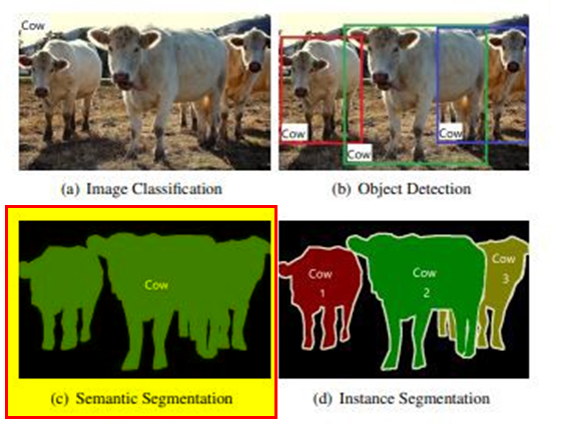
\includegraphics[width=0.75\textwidth]{semantic_segmentation_vs_others}
    \caption[Segmentation semantic]{Segmentation semantic\parencite[p.~1]{wu_recent_2019}}
    \label{fig:semantic_segmentation_vs_others}
 \end{figure}
\noindent Il existe différents cadres applicatifs pour l'entrainement de modèles \acrshort{ia}, tels que PyTorch ou TensorFlow. L'inconvénient est d'avoir à installer pour chacun leur propre environnement de développement et d'inférence, ce qui augmente les efforts et les coûts. Le cadre applicatif ONNX a été conçu pour pallier cette contrainte. En effet, il uniformise les architectures des modèles, et simplifie la mise en service grâce à l'installation d'un unique cadre applicatif. NVIDIA fournit avec le Jetson Nano une plateforme applicative qui supporte les modèles convertis au format ONNX, et offre donc une solution supportant l'interopérationabilité des modèles \acrshort{ia}. 
\subsection{Objectifs}
\noindent L'objectif principal de cet essai consiste a étudier la capacité du nano ordinateur du fabricant NVIDIA, le Jetson Nano \parencite{nvidia_jetson_2019}, à exécuter, en temps réel, une architecture de réseau de neurones pleinement connectés (\acrshort{fcnn}) entrainée à faire de la segmentation sémantique d'images et de vidéos de hautes résolutions qui sont perçues avec la caméra. Une seule classe sera extraite, celle représentant la piste multifonctionnelle. Les autres classes ne seront pas utilisées. Il semble important de préciser que l'objectif de l'essai n'est pas d'évaluer la précision (\acrshort{iou},  F1 score) de la segmentation sémantique, mais de déterminer, et ce en rapport avec les attentes du projet pour \acrshort{pjcci}, si la segmentation sémantique en temps réel d'une vidéo de haute qualité avec le Jetson Nano dans un mode opérationnel 24/7 est viable, et si les délimitations de la piste multifonctionnelle sont jugées acceptables pour être utilisée par un autre programme pour détecter les conditions de la surface.
\vspace{\baselineskip}
\\
\noindent Les sous-objectifs sont les suivants: 
\begin{itemize}
   \item Évaluer les limites de la plateforme, matérielle et applicative.
   \item Évaluer les moyens d'optimiser la plateforme d'un point de vue matériel et applicatif. 
   \item Évaluer la possibilité de pouvoir ré entrainer l'architecture sur le nano ordinateur dans une perspective d'apprentissage actif et continue.
   \item Ré entrainer une architecture \acrshort{fcnn} avec les images du site d'implémentation.
   \item Permettre un accès à distance sécurisé au nano ordinateur.
   \item Documenter l'approche, les tests, et les résultats;
\end{itemize}
\vspace{\baselineskip}
\noindent Il n'est pas planifier de faire des tests sur le site d'implémentation, ni s'intégrer avec d'autres programmes du projet pour \acrshort{pjcci}, par exemple pour détecter les conditions de la surface de la piste multifonctionnelle. 
\vspace{\baselineskip}
\\
\noindent Le premier sous-objectif est de déterminer quelles sont les limites de la plateforme, d'un point de vue matériel (\acrshort{gpu}, \acrshort{cpu}s, mémoire, transfert mémoire, consommation, etc.), mais aussi applicatif, d'un point de vue inférence. Cette phase du projet va permettre d'exécuter tel quel différents modèles d'architecture déjà existants, sans les ré entrainer, en tenant compte des éléments documentés dans la littérature \parencite{nguyen_mavnet_2019, zheng_real-time_2020, nvidia_jetson_2019-1}.
\vspace{\baselineskip}
\\
\noindent Un autre sous-objectif est d'optimiser ou d'adapter la plateforme, d'un point de vue matériel, mais aussi applicatif, afin d'avoir les meilleures performances et résultats possibles pendant l'inférence.
\vspace{\baselineskip}
\\
\noindent L'un des intérêts de l'\acrshort{ia} est de pouvoir améliorer constamment les modèles grâce au ré entrainment continue. L'essai va évaluer la possibilité de bénéficier de cet avantage directement sur le nano ordinateur en tentant de ré entrainer activement l'architecture avec des images de la piste multifonctionnelle re segmentées par un expert, et re générer un modèle plus précis, tout ceci en concurence avec l'inférence en temps réel. 
\vspace{\baselineskip}
\\
\noindent Comme les résultats devront être disponibles en tout temps, une connexion à distance sécurisée devra être mise en place. Cette connexion permettra aussi de pouvoir prendre le contrôle du nano ordinateur à distance et de l'administrer. En effet, le nano ordinateur sera déployé sur le site d'implémentation sans les périphériques standards, tel qu'un clavier, souris ou écran. Le type de réseau adéquat, soit Ethernet ou cellulaire (carte SIM réseau 3g/4g), sera évalué.
\vspace{\baselineskip}
\\
\noindent L'approche, les tests, et les résultats sont documentés. Il y aura beaucoup d'activités relatives à la conception et aux tests, le cheminement complet n'est pas fourni. Une synthèse est préférée et les informations les plus pertinentes sont incluses. Les détails de l'installation de l'environnement de développement et des applications, librairies et autres dépendances nécessaires sont inclus, ainsi que ceux de la configuration. Dans le cas où l'objectif principal n'est pas atteint, ou partiellement, la/les raison/s de l'échec sont spécifiées et des pistes de solutions potentielles proposées.

\section{Cadre théorique (état des connaissances, revue de la littérature) -- 5-9 pages}
Il y a deux sections, la première qui concernent le nano-ordinateur et ensuite la seconde, l'apprentissage profond et la segmentation sémantique.
\subsection{Cadre théorique au sujet du nano-ordinateur}
\par Voici le plan qui est utilisé pour rédiger le cadre théorique au sujet du nano-ordinateur.
\begin{itemize}
   \item historique et évolution; une brève présentation de l'historique des nano-ordinateurs, de leur apparition à leur place aujourd'hui.
   \par 
   \item usages; quelques exemples d'usages des nano-ordinateurs, dans un contexte professionnel.
   \par 
   \item architecture; brève présentation, fonctionnement et comparaison des architectures matérielles des nano-ordinateurs, leurs coûts, leurs avantages et limitations.
   \par 
\end{itemize}
\vspace{1\baselineskip}
\par 



\subsection{Cadre théorique au sujet de l'apprentisage profond et de la segmentation sémantique -- 3-5 pages}
\noindent La segmentation sémantique d'images ou de vidéos est une technique de télédétection du domaine de la vision par ordinateur. Elle permet de délimiter (segmenter) différentes parties (sémantique) d'une image. Les méthodes de segmentation ont été améliorées ces dernières années par les récentes avancées dans le domaine de l'apprentissage profond. 
\begin{figure}[H]
   \centering
   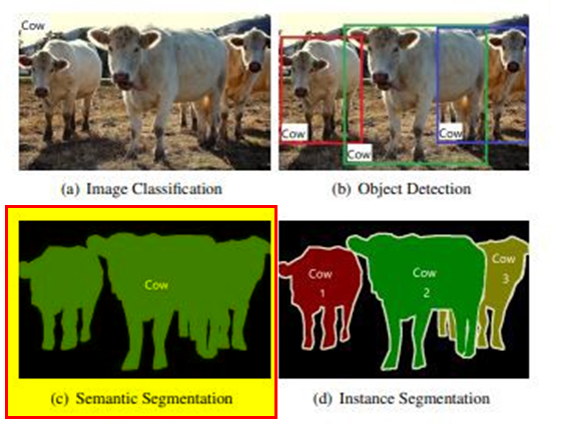
\includegraphics[width=0.75\textwidth]{semantic_segmentation_vs_others}
   \caption[Segmentation semantic]{Segmentation semantic\cite[p.~1]{wu_recent_2019}}
   \label{fig:semantic_segmentation_vs_others}
\end{figure}
\noindent L’apprentissage profond est un sous-domaine de celui de l'apprentissage machine qui est un sous-domaine de celui de l'intelligence artificielle. 
\begin{figure}[H]
   \centering
   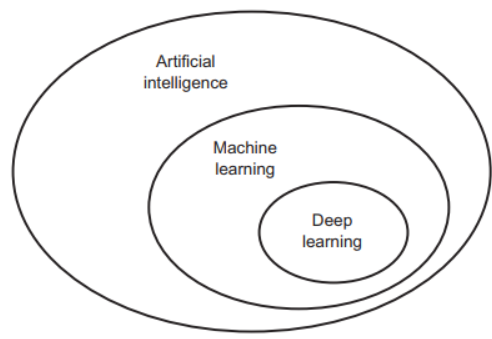
\includegraphics[width=0.5\textwidth]{Deep_Learning_with_Python.pdf}
   \caption[Relation entre \acrlong{ia}, \acrlong{am} et \acrlong{ap}]{Relation entre \acrlong{ia}, \acrlong{am} et \acrlong{ap} \cite[p.~4]{chollet_deep_2018}}
   \label{fig:ia_ml_ap}
\end{figure}
\noindent Les concepts de l'\lowercase{\acrlong{ia}} (AI) existent depuis les années 1950 \cite[p.~4]{chollet_deep_2018} \cite[p.~1]{alom_history_2018}, et ont continué à se développer par vague, jusqu'à leur nouvelle popularité des 15 dernières années. En effet, trois raisons principales ont permis à ce domaine de renaitre de nouveau \cite[p.~20]{chollet_deep_2018}: la capacité et la puissance des machines; des jeux de données plus larges; des algorithmes plus avancés. Les deux moments clés, preuves de cette renaissance, sont: 1) la possibilité d'entrainer des architectures de réseaux de neurones profonds (DNN) (2006) \cite[p.~6]{alom_history_2018}; et 2) l'architecture du réseau de neurones convolutionels AlexNet permet de  gagner le challenge ImageNet contre les approches traditionnelles\cite[p.~11]{alom_history_2018}. 
\vspace{\baselineskip}
\\
\noindent En 2016 \cite[p.~14]{alom_history_2018}, l'architecture \acrshort{fcn} (\acrlong{fcn}, réseau (de neurones) convolutionnel entier) a permis aux taches réservées à la segmentation d'images d'être plus efficace que les méthodes traditionnelles de la vision par ordinateur. Cette nouvelle méthode s'applique désormais à tous les domaines connexes à l'analyse d'images, tels que l'imagerie médicale, la conduite autonome de véhicules, la robotique, la télédétection d'images satellites, la sécurité par caméra vidéo, l'agriculture de haute précision. Aujourd'hui, elle peut s'exécuter en temps réel sur des systèmes embarqués proche des données. 

\section{Matériel et méthodes}
\subsection{Site d'étude - 1 page}
\par Tel que trouvé dans le rapport détaillé sur le projet pilote d'entretien hivernal de la piste multifonctionnelle du pont Jacques-Cartier \cite{pjcci_rapport_2018}, la piste multifonctionnelle du pont Jacques Cartier relie Montréal intramuros, proche de la station de métro Papineau, et la rive sud, à Longueuil, proche de la station de métro Longueuil et le terminal de bus. Elle est longue d'une distance de 2.7km et est située d'un seul côté du pont, côté sud. Elle est surtout utilisée par les cyclistes, et moindrement par les passants. 
Sa configuration est bien particulière \cite{pjcci_fiche_2018}: elle ne longe pas la route adjacente sur toute sa longueur; elle est interrompue par une voie de sortie de l'île Notre-Dame; des chicanes sont disposés à certains endroits; sa largeur varie entre 2.5 et 1.8 mètre; elle possède une pente assez prononcée à certains moments; il y a des courbes assez serrées.
Elle est fermée l'hiver par mesure de sécurité. Elle est ouverte au début du printemps jusqu'au début de l'hiver, lorsque les conditions ne nécessitent pas d'entretien.
\label{pjcci_vueaerienne}
\begin{figure}[H]
    \centering
    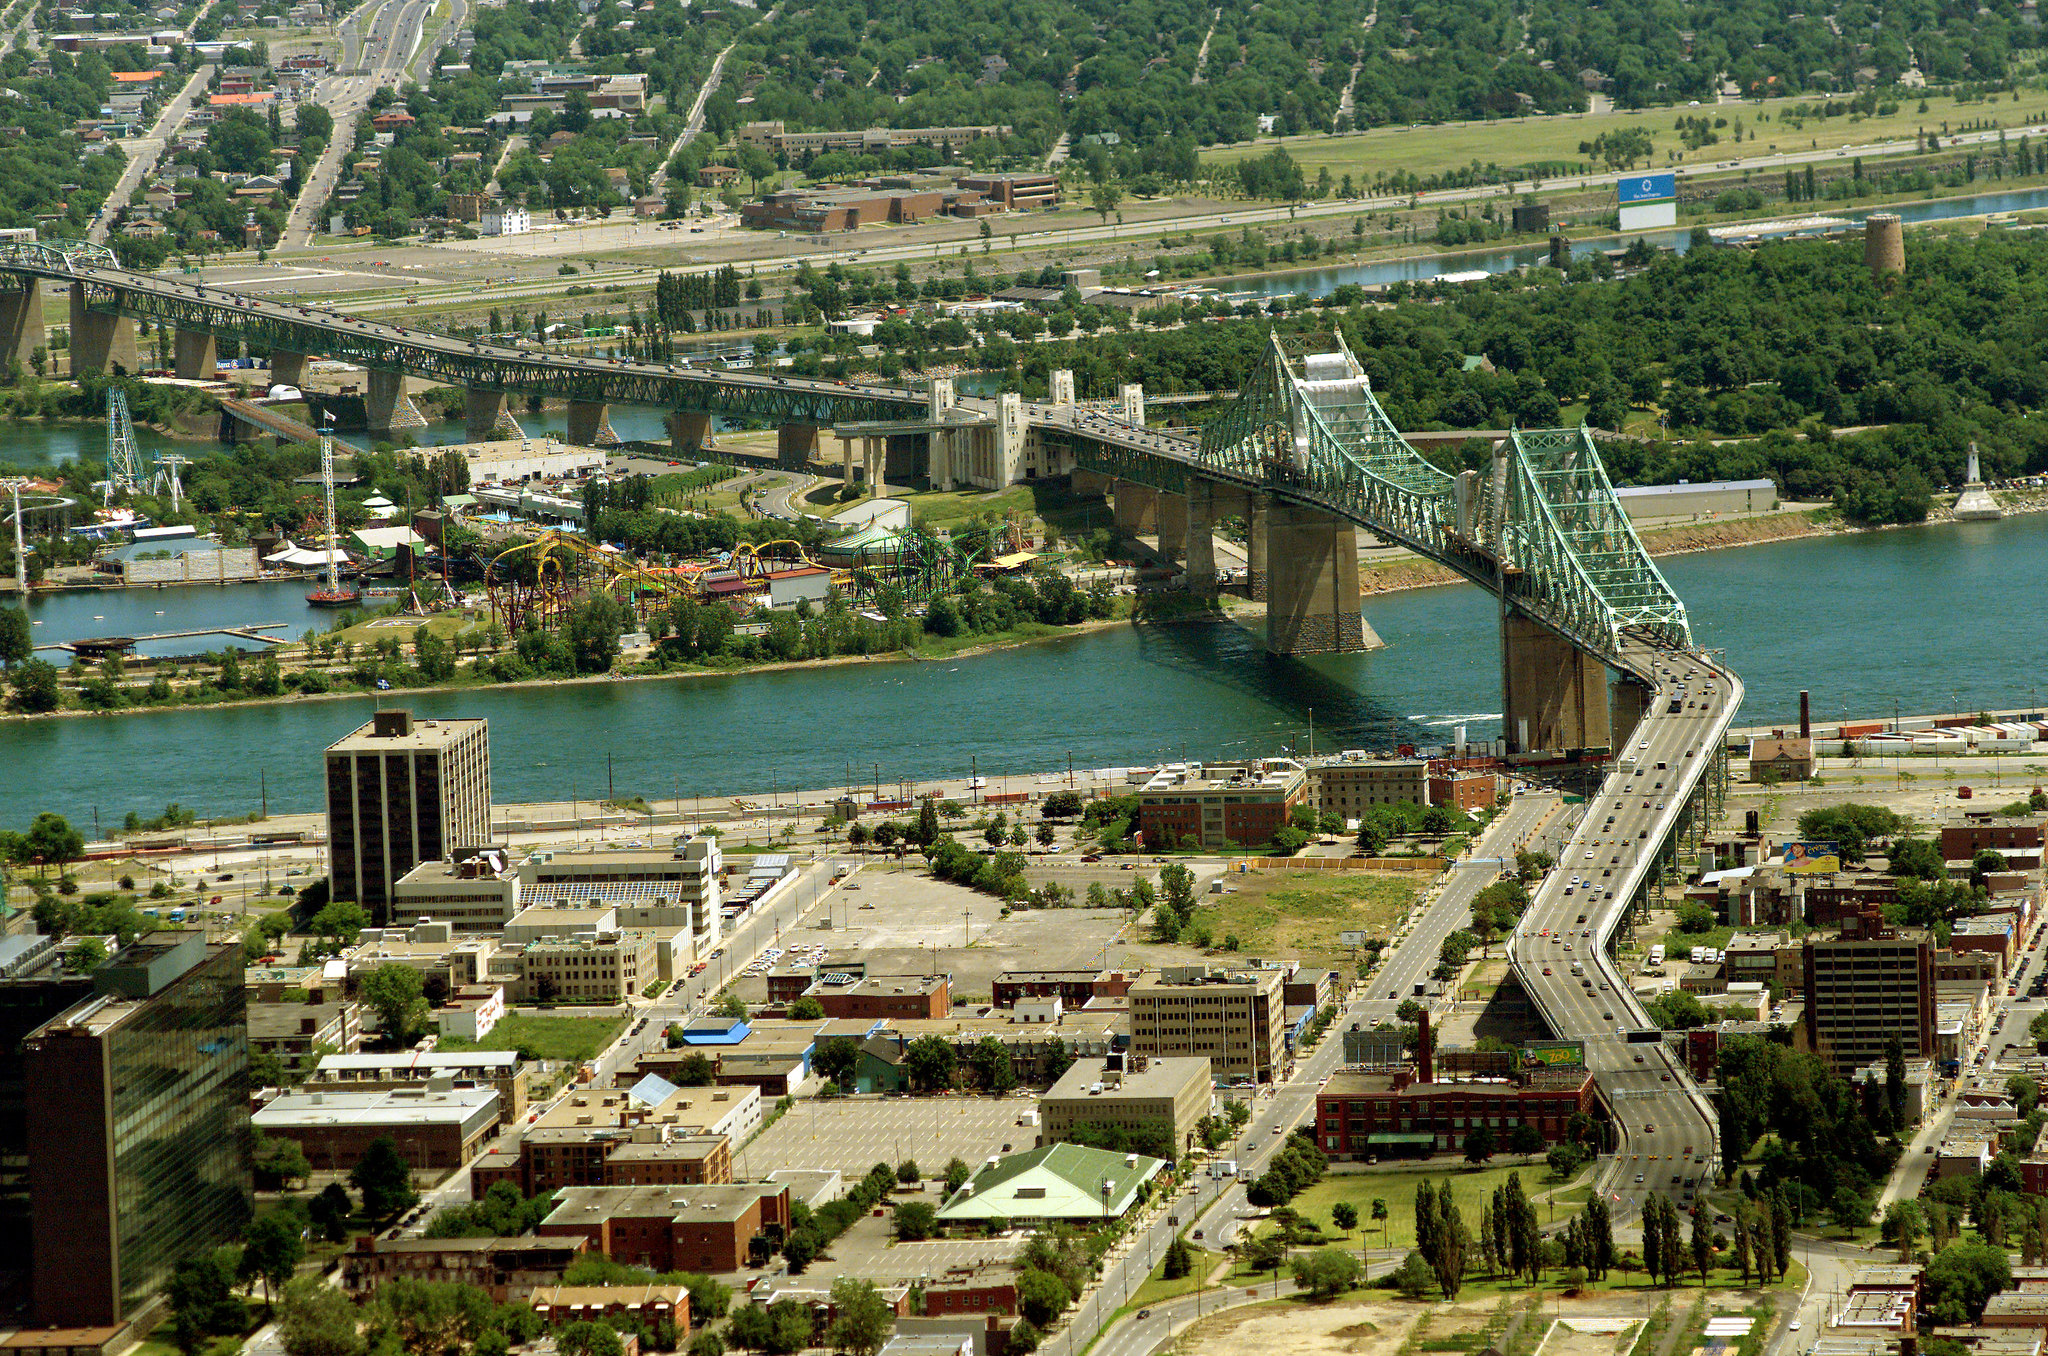
\includegraphics[width=1.0\textwidth]{pjcci_vueaerienne}
    \caption{Vue aérienne du pont Jacques-Cartier}
    \label{fig:pjcci_vueaerienne}
\end{figure}
\label{alamy_com_vueaerienne}
\begin{figure}[H]
    \centering
    
\includegraphics[width=1.0\textwidth]{alamy_com_vueaerienne}
    \caption{Vue aérienne du pont Jacques-Cartier}
    \label{fig:alamy_com_vueaerienne}
\end{figure}
\label{carte_site_etude}
\begin{figure}[H]
    \centering
    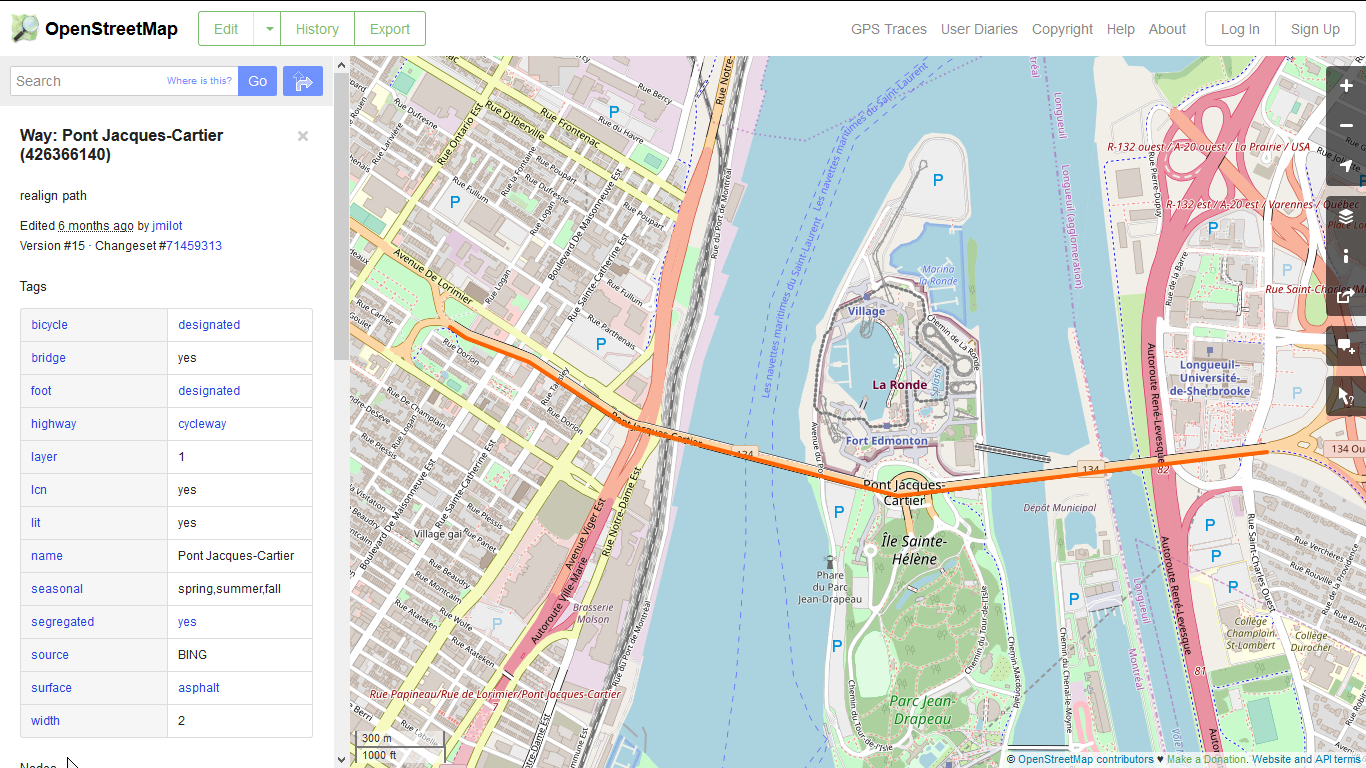
\includegraphics[width=1.0\textwidth]{carte_site_etude}
    \caption{Carte du site d'implantation : le pont Jacques-Cartier et la piste multifonctionnelle en orange sur le pont}
    \label{fig:carte_site_etude}
\end{figure}
\label{Fiche_piste-multi_pont_JC_FR_vfinale_2018-10-10}
\begin{figure}[H]
    \centering
    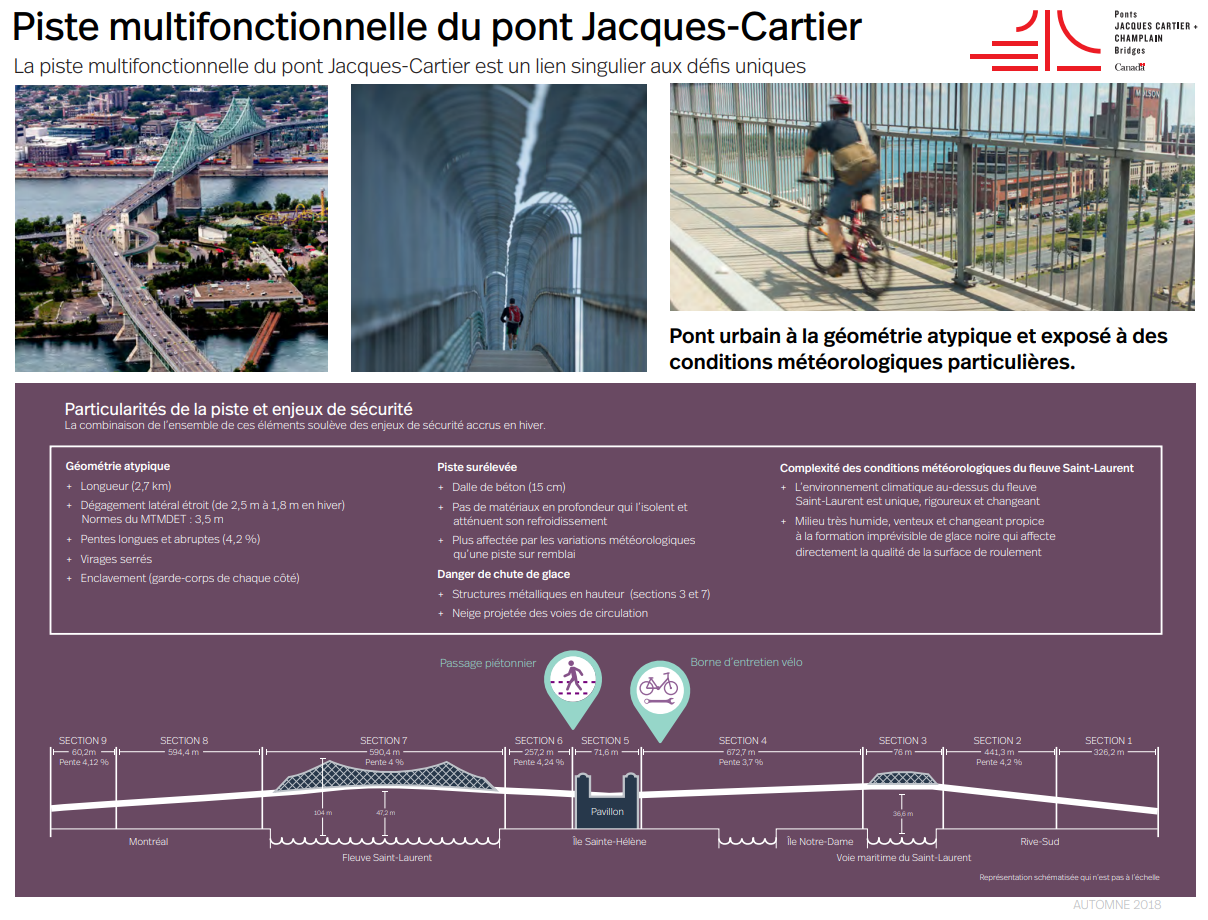
\includegraphics[width=1.0\textwidth]{Fiche_piste-multi_pont_JC_FR_vfinale_2018-10-10}
    \caption{Schéma de la configuration de la piste multifonctionnelle}
    \label{fig:Fiche_piste-multi_pont_JC_FR_vfinale_2018-10-10}
\end{figure}
\subsection{Données -– 3-4 pages}
\par Voici le plan qui est utilisé pour rédiger au sujet des données.
\begin{itemize}
   \item Présentation des réseaux de neurones qui seront utilisés dans le cadre de l’essai, leurs caractéristiques.
   \item Présentation des sources de données (images) qui seront utilisées pour l'apprentissage, la validation et les tests des réseaux de neurones pour le ré-entrainement.
   \item Présentation des sources de données (images et vidéos) qui seront utilisées pour l'inférence.
\end{itemize}

\paragraph{Données}\label{metho:data}

\begin{itemize}
   \item Précision des différentes sources consultées:
      \begin{itemize}
         \item Les ressources mises à disposition par le constructeur du Jetson nano, NVIDIA, font référence à des jeux de données qui sont disponibles publiquement.
         \item En complément des ressources de NVIDIA, deux références scientifiques seront principalement étudiées, car leurs recherches ont été faites avec le Jetson nano (\cite{nguyen_mavnet_2019} et \cite{chong_real-time_1992}). Beaucoup de références ont été publiées ces deux dernières années sur le sujet de la segmentation sémantique, ils existent donc de multiples alternatives inspirantes.
         \item Internet est une mine de données. Il existe des forums et des blogues dans lesquels des utilisateurs publient leurs expérimentations de la segmentation sémantique en temps réel avec le Jetson nano (\cite{dustin_realtime_2019}), ou plus génériquement la segmentation sémantique. Des sites comme "modelzoo.co" ou "kaggle.com" sont des entrepôts de données. Une autre option est d'effectuer une recherche d'images ou de vidéos de la piste multifonctionnelle du pont Jacques-Cartier via les sites de recherche tels que Google. 
         \item L'Association des piétons et cyclistes du pont Jacques-Cartier existe depuis de nombreuses années pour promouvoir le transport actif et conserver la piste multifonctionnelle du pont Jacques Cartier ouverte durant l'hiver. Ils fournissent, via leurs sites Internet, des collections de vidéos et d'images qui pourraient être utilisées. Il serait aussi possible d'entrer en contact avec l'association et leur demander de prendre de nouvelles vidéos. Voir "http://pontjacquescartier365.com", et\\"https://www.flickr.com/photos/pontjacquescartier".
         \item Une autre possibilité serait d'hériter des acquisitions faites par un autre étudiant de l'université de Sherbrooke, soit déjà archivée, soit collectée prochainement. Mon directeur de projet Mickaël G. m'a informé qu'un étudiant de Sherbrooke va avoir besoin de collecter le trafic automobile sur le campus de l'Université de Sherbrooke, à Sherbrooke. 
         \item Enfin il y a l'acquisition des vidéos spécifiquement pour le projet PJCCI. Comme il n'y a aucune date de planifiée pour la capture des vidéos, l'essai devra s'arranger pour dépendre le moins possible d'elles durant la préparation et le développement, et s'attendre à les recevoir pour le ré-apprentissage et les tests, en fin d'essai.
         \item Tout au long de l'essai, mon directeur Mickaël sera une ressource importante afin de vérifier que les sources de données, les prétraitements et les traitements sont adéquats aux attentes du projet pour PJCCI.
      \end{itemize}
   \item Récapitulatif des jeux de données utilisés pour l'essai, grâce à un tableau: les réseaux de neurones et le nom des jeux de données d’imageries et de vidéos respectifs; leur source; le nombre d’images; leur résolution, leur nombre d'images par secondes dans le cas des vidéos.
   \item Présentation des images utilisées pour le ré-entrainement des modèles, la validation et les tests; les traitements nécessaires des vidéos et des images. 
   \item Présentation des vidéos et des images qui seront utilisées pour l'inférence; les traitements nécessaires des vidéos et des images.
   \item Mention de la méthodologie d'acquisition des nouvelles données sur le site d'étude (même si potentiellement elles ne seront pas utilisées pendant l'essai ?).
\end{itemize}

\myparagraph{Approche prévue pour le traitement des données}
\par Il y a deux phases à cet essai: l'inférence avec des modèles déjà prêts et l'inférence avec des modèles ré-entrainés. Les données utilisées par l'inférence sont des vidéos (d'une certaine résolution et d'un certain nombre d'images pas seconde), et celles pour l'entrainement sont des images. Dans les deux cas, les images pour l'entrainement ou l'inférence doivent être d'une taille bien précise, celle avec laquelle le modèle a été, ou sera, entrainé. La résolution et la qualité de l'image-vidéo seront nivelées vers le bas afin de déterminer la limite inférieure acceptable pour la détection la plus efficace et fiable possible. La résolution et le nombre d'images par seconde de la vidéo sont contrôlés par le logiciel ("driver" en anglais) de la caméra, et sont configurables. 
\par Tout cela signifie que les vidéos ou nouvelles images devront être traités pour répondre à une certaine taille et résolution requise par le modèle, tout en conservant une qualité élevée (nombre de pixels, niveaux de couleurs). De nouvelles images pour l'entrainement seront extraites des vidéos, et annotées. 
\par Certains framework d'apprentissage profond (par exemple "Keras") offrent l'option d'augmenter automatiquement le jeu de données avec des techniques d'augmentation de données (par exemple la rotation, le redimensionnement, l'effet miroir), ce qui est très utile et non négligeable.

\par Voici le tableau de synthèse des données, incluant la référence avec leur réseaux de neurones.
{
   \clearpage 
   \newpage
   \begin{landscape}
   \newcounter{magicrownumbers}
   \newcommand\rownumber{\stepcounter{magicrownumbers}\arabic{magicrownumbers}}
   % \centering
   \vspace{0.3em} % Adjust the height of the space between caption and tabular
   \begin{longtable}[t]{@{}p{1em}|p{15em}p{35em}@{}} % p{15em}p{35em} with landscape
      \caption{Tableau des données}\label{tab:datasets}\\
      & \textbf{Spécification} & \textbf{Description}\\
      \hline
      \endfirsthead
      & \textbf{Spécification} & \textbf{Description}\\
      \hline
      \endhead
      \endfoot
      \endlastfoot
      \hline
      \rownumber & \begin{tabular}[t]{@{}p{15em}@{}}
         réseau: U-Net\\jeu de données: Membrane (origine isbi challenge)\\nombre d'images: 30\\résolution/s: 512x512
      \end{tabular} & \begin{tabular}[t]{@{}p{35em}@{}}
         C'est le jeu de données pour le réseau U-Net. Il est utilisé dans le benchmark de NVIDIA pour l'inférence avec le Jetson nano. Les images sont de type médicale.\\
         À noter que le framework "Keras" s'occupe de l'augmentation de données.\\
         https://github.com/zhixuhao/unet/tree/master/data/membrane\\
      \end{tabular}\\
      \hline
      \rownumber & \begin{tabular}[t]{@{}p{15em}@{}}
         réseau: SegNet\\jeu de données: CamVid\\vidéos: 10 minutes\\résolution/s: HD
      \end{tabular} & \begin{tabular}[t]{@{}p{35em}@{}}
         SegNet est un réseau qui a été créé pour la segmentation sémantique de vidéos. Il a été entrainé avec le jeu de données de CamVid, qui procurents des vidéos de la route avec la méme perspective que le conducteur du véhicule. Un modèle entrainé est disponible pour le Jetson nano.\\
         https://github.com/PengKiKi/camvid\\
      \end{tabular}\\
      \hline
      \rownumber & \begin{tabular}[t]{@{}p{15em}@{}}
         réseau: MFANet\\jeu de données: Cityscapes\\nombre d'images: 5000\\résolution/s: 1280x1024
      \end{tabular} & \begin{tabular}[t]{@{}p{35em}@{}}
         MFANet est un réseau qui a été créé en 2019 pour la segmentation sémantique sur des appareils tel que le Jetson nano. Il a été entrainé avec le jeu de données de Cityscapes, qui procurents des images de scènes urbaines. Différentes stratégies d'augmentation de données sont utilisées. Des tests ont été fait avec le Jetson nano.\\
         leejy@ustb.edu.cn\\
      \end{tabular}\\
      \hline
      \rownumber & \begin{tabular}[t]{@{}p{15em}@{}}
         réseau: MAVNet\\jeu de données: Penstock\\nombre d'images: 135\\résolution/s: 1280x1024
      \end{tabular} & \begin{tabular}[t]{@{}p{35em}@{}}
         C'est l'un des deux jeux de données pour le réseau MAVNet. Les images sont celles de "conduites forcées", des voies d'eau de régulation, et sont préparées pour la segmentation sémantique. Des tests ont été fait avec le Jetson nano.\\
         https://github.com/tynguyen/MAVNet/tree/master/data/TN\_penstock\\
      \end{tabular}\\
      \hline
      \rownumber & \begin{tabular}[t]{@{}p{15em}@{}}
         réseau: MAVNet\\jeu de données: Penstock\\nombre d'images: 135\\résolution/s: 1280x1024
      \end{tabular} & \begin{tabular}[t]{@{}p{35em}@{}}
         C'est l'un des deux jeux de données pour le réseau MAVNet. Les images sont celles de drones volant à l'intérieur d'un bâtiment, et préparées pour la segmentation sémantique. Des tests ont été fait avec le Jetson nano.\\
         https://github.com/tynguyen/MAVNet/tree/master/data/perch\_drone\\
      \end{tabular}\\
      \hline
      \rownumber & \begin{tabular}[t]{@{}p{15em}@{}}
         réseau: RESNet18\\jeu de données: Cityscapes\\nombre d'images: 25 000\\résolution/s: 360x720, 512x256, 1024x512, 2048x1024
      \end{tabular} & \begin{tabular}[t]{@{}p{35em}@{}}
         Cityscapes est un jeu de données qui fournit des images de rues spécifiquement destinées pour la segmentation sémantique. Il peut être utilisé par de nombreux réseaux. RESNet18 a été entrainé avec ce jeu et est disponible en diverses résolutions pour le Jetson Nano.\\
         https://github.com/tynguyen/MAVNet/tree/master/data/perch\_drone\\
      \end{tabular}\\
      \hline
      \rownumber & \begin{tabular}[t]{@{}p{15em}@{}}
         réseau: RESNet18\\jeu de données: DeepScenes\\nombre d'images: 15 000\\résolution/s: 576x320, 864x480 
      \end{tabular} & \begin{tabular}[t]{@{}p{35em}@{}}
         DeepScene propose un modèle et un jeu de données. Le modèle est entrainé avec différents jeux de données, comme Cityscpapes, SUN-RGBD, Synthia. Le jeu de données fournit des images de forêt, qui est destinée pour la segmentation sémantique. RESNet18 a été entrainé avec ce jeu et est disponible en deux  résolutions pour le Jetson Nano.\\
         http://deepscene.cs.uni-freiburg.de\\
      \end{tabular}\\
      \hline
      \rownumber & \begin{tabular}[t]{@{}p{15em}@{}}
         réseau: RESNet18\\jeu de données: Multi-Human\\nombre d'images: 25 043\\résolution/s: 512x320, 640x360
      \end{tabular} & \begin{tabular}[t]{@{}p{35em}@{}}
         Le jeu de données Multi-Human fournit des images contenant des humains, et qui est destinée pour la segmentation sémantique. RESNet18 a été entrainé avec ce jeu et est disponible en deux résolutions pour le Jetson Nano.\\
         https://lv-mhp.github.io/dataset\\
      \end{tabular}\\
      \hline
      \rownumber & \begin{tabular}[t]{@{}p{15em}@{}}
         réseau: RESNet18\\jeu de données: Pascal VOC\\nombre d'images: 11 530\\résolution/s: 320x320, 512x320 
      \end{tabular} & \begin{tabular}[t]{@{}p{35em}@{}}
         Le jeu de données Pascal VOC fournit des images de classes variées tel que des personnes, des animaux, des véhicules, et des objets classiques, et qui peut être utilisé pour la segmentation sémantique. RESNet18 a été entrainé avec ce jeu et est disponible en deux résolutions pour le Jetson Nano.\\
         http://host.robots.ox.ac.uk/pascal/VOC/voc2012/index.html\\
      \end{tabular}\\
      \hline
      \rownumber & \begin{tabular}[t]{@{}p{15em}@{}}
         réseau: RESNet18\\jeu de données: SUN RGB-D\\nombre d'images: 10 335\\résolution/s: 512x400, 640x512
      \end{tabular} & \begin{tabular}[t]{@{}p{35em}@{}}
         Le jeu de données SUN RGB-D fournit des images de scènes d'intérieur de maison, et qui est destiné pour la segmentation sémantique. RESNet18 a été entrainé avec ce jeu.\\
         https://synthia-dataset.net\\
      \end{tabular}\\
      \hline
      \rownumber & \begin{tabular}[t]{@{}p{15em}@{}}
         réseau: DeepScene\\jeu de données: Synthia\\nombre d'images: 220 000\\résolution/s: 1280x760
      \end{tabular} & \begin{tabular}[t]{@{}p{35em}@{}}
         Le jeu de données Synthia fournit des images (et vidéos) de scènes de rue comme celui de Cityscapes, et qui est destiné pour la segmentation sémantique. DeepScene a été entrainé avec ce jeu. Il n'a pas été testé avec le Jetson Nano.\\
         http://3dvision.princeton.edu/datasets.html\\
      \end{tabular}\\
      \hline
      \rownumber & \begin{tabular}[t]{@{}p{15em}@{}}
         jeu de données: Association des piétons et cyclistes pont Jacques-Cartier\\nombre d'images: 313\\résolution/s: variées
      \end{tabular} & \begin{tabular}[t]{@{}p{35em}@{}}
         L'Association des piétons et cyclistes du pont Jacques-Cartier a une collection d'images et de vidéos de la piste multifonctionnelle du pont Jacques-Cartier. Ce n'est pas un jeu de données qui est prêt à être utilisé pour l'apprentissage tel-quel, il doit être préparé. Mais c'est une source de données qui est très importante pour l'essai. Il est envisagé de contacter l'association au besoin afin de leur demander leur collaboration pour la collecte d'autres d'images ou vidéos.\\
         https://www.flickr.com/photos/pontjacquescartier\\
         http://pontjacquescartier365.com/videos-pont-jacques-cartier\\
      \end{tabular}\\
      \hline
      \rownumber & \begin{tabular}[t]{@{}p{15em}@{}}
         jeu de données: images et vidéo sur Internet\\nombre d'images: entre 30-50\\résolution/s: variées
      \end{tabular} & \begin{tabular}[t]{@{}p{35em}@{}}
         Internet est une source de données non négligeable en terme de données. Quelques images et vidéos de la piste multifonctionnelles du pont Jacques-Cartier, autres que celles fournies par L'Association des piétons et cyclistes du pont Jacques-Cartier, sont disponibles. Ce n'est pas un jeu de données qui est prêt à être utilisé pour l'apprentissage tel-quel, il doit être préparé. Mais c'est une source de données qui est très importante pour l'essai.\\
         https://google.ca\\
      \end{tabular}\\
      \hline
      \rownumber & \begin{tabular}[t]{@{}p{15em}@{}}
         jeux de données: Kaggle
      \end{tabular} & \begin{tabular}[t]{@{}p{35em}@{}}
         Le site Kaggle offre une vingtaine de jeux de données offert par la communauté pour faire de la segmentation sémantique, et qui sont prêt à être utilisé. Les jeux de données n'ont pas été évalués.\\
         https://www.kaggle.com/search?q=%22semantic+segmentation%22+in%3Adatasets\\
      \end{tabular}\\
      \hline
   \end{longtable}
   \end{landscape}
   \clearpage
   \newpage
}

\subsection{Matériel et logiciels –- 2-3 pages}
\par Voici le plan qui est utilisé pour rédiger au sujet du matériel.
\begin{itemize}
   \item Présentation du nano-ordinateur qui sera utilisé, le NVIDIA Jetson nano;
   \item Usage du nano-ordinateur durant l'essai.
\end{itemize}

\par L'objet d'étude de cet essai est un nano-ordinateur. Un nano-ordinateur est un ordinateur miniaturisé en taille, mais aussi limité en capacité. Il existe différents fabricants et modèles, de caractéristiques techniques variées, pour répondre à différents besoins. Le dernier né est le modèle "Jetson nano" du fabricant "NVIDIA", disponible depuis juin 2019 au prix très abordable de 99\$US. La compagnie NVIDIA a conçu ce matériel spécialement pour différentes applications d'inférence de modèles d'apprentissage profond sur une plateforme mobile (drone) ou proche des données ("edge" en anglais). Ce modèle a été choisi afin de répondre à l'intérêt que suscitent ses capacités et ses limites. Une image du Jetson nano et un tableau de ses caractéristiques techniques seront ajoutés. 
\par L'architecture matérielle sera étudiée et présentée avec l'aide d'images, de diagrammes et de textes explicatifs. Les éléments clés seront identifiés.
\par Afin d'optimiser les performances du Jetson nano, une recherche des périphériques les plus adaptés pour répondre aux besoins de performance (et de budget) de l'essai est essentielle, telle que l'alimentation, le stockage, la caméra. Des images des périphériques seront incluses, et les caractéristiques principales seront présentées dans des tableaux.
\par Il est à noter que le NVIDIA Jetson nano est déjà en ma possession. La liste des équipements est en cours et sera commandée par le collaborateur "Vision météo".

\paragraph{Logiciels -– 1-2 pages}
\par De même que pour les périphériques, les logiciels qui seront utilisés seront résumés dans un tableau, où il sera indiqué leur nom, le type de licence, leur version, leurs avantages et limitations, comme pour le système d'exploitation, l'environnement de développement pour l'apprentissage profond, l'inférence, les logiciels de traitements vidéos et d'images. 
\begin{itemize}
   \item Présentation du système d'exploitation qui sera installé;
   \item Présentation des frameworks d’apprentissage profond qui vont être utilisés (PyTorchm torchvision);
   \item Présentation des librairies pour d'inférence (TensorRT, onnx);
\end{itemize}
\vspace{1\baselineskip}
\par 
\subsection{Méthodologie –- 10-15 pages}
\par Voici à très haut niveau les grandes étapes de cet essai:
\label{methodologie_haut_niveau}
\begin{figure}[H]
    \centering
    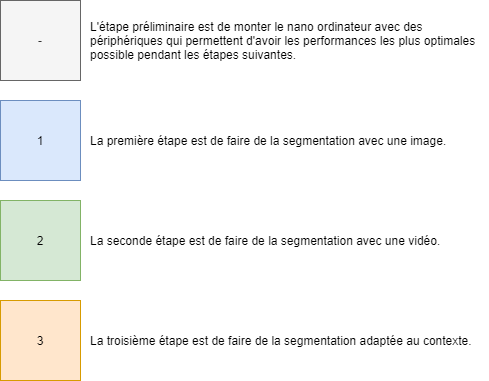
\includegraphics[width=0.75\textwidth]{methodologie_haut_niveau}
    \caption{Organigrame de la méthodologie à haut niveau}
    \label{fig:methodologie_haut_niveau}
\end{figure}
\par Pour y parvenir, la méthodologie suivante a été suivie et permet d'évaluer les performances de base de la segmentation sémantique avec le nano ordinateur.
\label{methodologie_simple}
\begin{figure}[H]
    \centering
    
\includegraphics[width=0.65\textwidth]{methodologie_simple}
    \caption{Organigrame de la méthodologie pour évaluer les performances}
    \label{fig:methodologie_simple}
\end{figure}
\par Si chacun des blocs est explosé, chacun d'eux s'organise autour des activités suivantes: 
\label{methodologie_simple_details}
\begin{figure}[H]
    \centering
    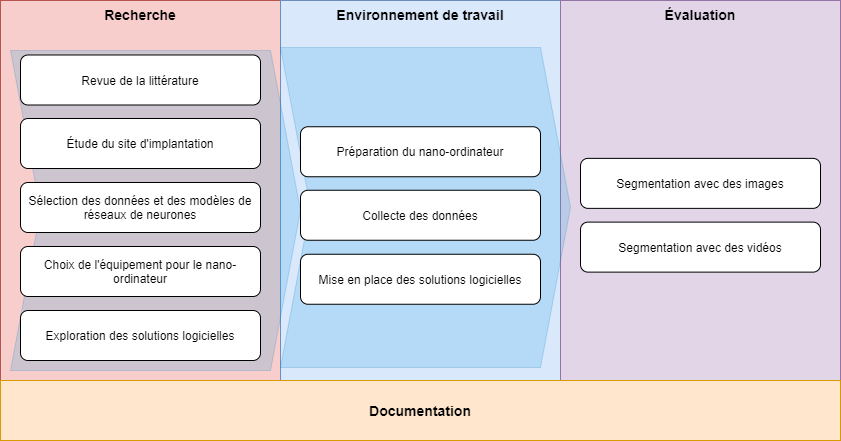
\includegraphics[width=1.0\textwidth]{methodologie_simple_details}
    \caption{Organigramme des détails de la méthodologie pour évaluer les performances}
    \label{fig:methodologie_simple_details}
\end{figure}
\par Si l'évaluation est probante, la méthodologie se verra bonifiée par des étapes d'adaptation et de traitement. 
\label{methodologie_complexe}
\begin{figure}[H]
    \centering
    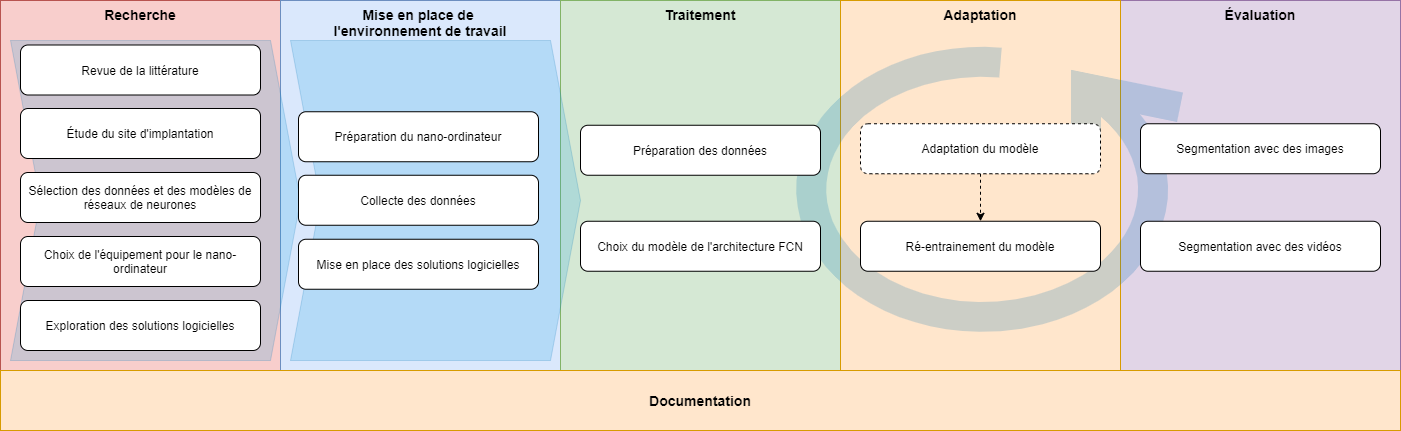
\includegraphics[width=0.75\textwidth]{methodologie_complexe}
    \caption{Organigramme de la méthodologie pour évaluer les performances après une phase d'adaptation théorique}
    \label{fig:methodologie_complexe}
\end{figure}
\par Mais sincèrement dans la pratique la méthodologie ressemblera plus à celle-ci: 
\label{methodologie_complexe_realiste}
\begin{figure}[H]
    \centering
    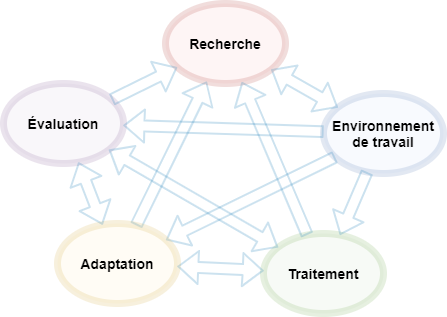
\includegraphics[width=0.65\textwidth]{methodologie_complexe_realiste}
    \caption{Organigramme de la méthodologie pour évaluer les performances après une phase d'adaptation réaliste}
    \label{fig:methodologie_complexe_realiste}
\end{figure}
\par Si chacun des blocs est explosé, chacun d'eux s'organise autour des activités suivantes: 
\label{methodologie_complexe_details}
\begin{figure}[H]
    \centering
    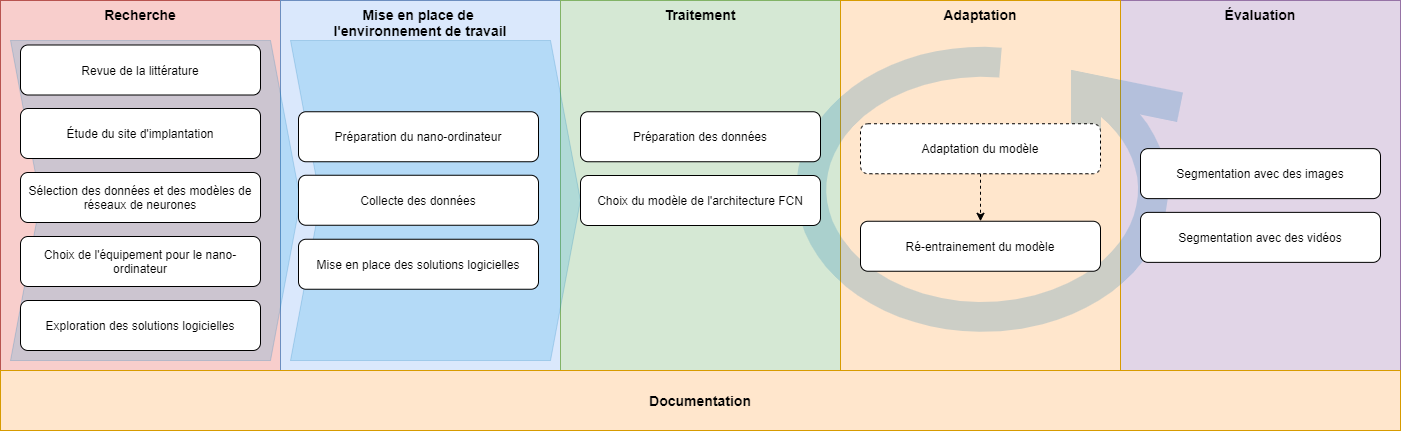
\includegraphics[width=1.0\textwidth]{methodologie_complexe_details}
    \caption{Organigramme des détails de la méthodologie pour évaluer les performances après une phase d'adaptation}
    \label{fig:methodologie_complexe_details}
\end{figure}
\par Les phases de la méthodologie présentée dans l'organigramme de la figure \ref{fig:methodologie_complexe_details} peuvent être résumées de la façon suivante:
\begin{itemize}
   \item Recherche des références, des modèles et des données, ainsi que l'équipement pour le nano ordinateur et des logiciels nécessaires.
   \item Installation sur le nano ordintaeur le système d'exploitation, l'environnement de développement et de tests pour l'inférence.
   \item Itération entre les étapes suivantes:
   \begin{itemize}
      \item Inférence avec le nano ordinateur en utilisant les modèles et les sources de données sélectionnées.
      \item Adaptation des modèles à différentes résolutions d'images et à la zone d'étude.
      \item Traitement des données afin de les adapter au requis des modèles.
   \end{itemize}
\end{itemize}
\par Finalement, il est à noter  que le cheminement de l'essai a été entièrement documenté pendant tout le déroulement de l'essai.
\subsection{Documentation}
\par La méthodologie a été entièrement documenté pendant tout le déroulement de l'essai. Elle se retrouve pour référence dans un blog publique sur le site de "github.io" \footnote{\url{https://vince7lf.github.io/}}. Cette méthodologie de documentation permet entre autre, de très facilement documenter, de ne pas perdre des notes très importantes, de suivre le cheminement, de pouvoir retrouver des notes, mêmes si elles ont été effacées ou modifiées, puisque toute modification est sauvegardée dans un repository Git.
\par Par ailleur, tous les documents de rédaction LaTeX, les images, les scripts et code source qui ont été utiles et utilisés durant l'essai ont été géré dans un repository Git publique avec "github.com" \footnote{\url{https://github.com/vince7lf/gae724}}. 
\par Ces sources d'information viennent bonifier grandement ce rapport et il est même recommandé de s'y référer pour atteindre un certains niveau détails et de compréhension. 
\subsection{Recherche}

\subsubsection{Revue de littérature}
\noindent La recherche s'est concentrée sur des références traitantes des concepts du sujet de l'essai : la segmentation sémantique, le temps réel, et les nano ordinateurs. Le premier objectif a été de trouver si des études avaient déjà expérimenté le nano ordinateur, en particulier pour la segmentation de vidéos en temps réel. Pendant cette recherche, j'en ai profité pour effectuer une révision de l'évolution des réseaux de neurones convolutionnels entiers (\acrshort{fcn} \acrlong{fcn})  et des différentes architectures, et chercher d'autres solutions de détection de la route en temps réel grâce au \acrshort{fcn}. 
\vspace{\baselineskip}
\\
\noindent Il a été assez compliqué de trouver des références intégrant les nano ordinateurs. Comme l'objectif de l'essai est de valider les performances d'un nano ordinateur bien spécifique, les mots-clés "NVIDIA Jetson Nano" font partie de la stratégie de recherche. 
\vspace{\baselineskip}
\\
\noindent Les réseaux de neurones convolutifs entiers (\acrshort{fcn}) sont implicitement inclus dans les résultats puisque c'est le "state-of-art" actuellement pour répondre au besoin de la segmentation sémantique d'images.
\vspace{\baselineskip}
\\
\noindent Plus de 75 références ont été collectées. Une quarantaine ont été sélectionnées. Cette sélection peut se décomposer en trois catégories : les références se rapprochant le plus du sujet de l'essai; l'histoire et les antécédents des réseaux de neurones; du matériel éducatif pour étudier et manipuler les réseaux de neurones.
\vspace{\baselineskip}
\\
\noindent Je me suis intéressé aux références des années les plus récentes, autour de 2020, 2019 et 2018, car les avancées dans le domaine des réseaux de neurones sont très rapides. Par curiosité je suis allé aussi parfois voir dans les années bien plus éloignées, comme 1998, ou j'ai trouvé un article proposant une solution pour prédire la température de la surface de la route avec des réseaux de neurones.
\vspace{\baselineskip}
\\
\noindent Je n'ai pas pu trouver de références spécifiquement pour la déduction de l'état de la surface (mouillé, gelée, etc.) d'une piste multifonctionnelle (vélo, piéton). 
\vspace{\baselineskip}
\\
\noindent Il est intéressant de noter que la banque de données SCOPUS retourne plus de 11,000 documents avec l'expression "segmentation AND "real-time"". Il y en a plus de 700 uniquement pour l'année 2019. 
\subsubsection{Étude du site d'implantation}
\par Le nano ordinateur est destiné à être déployé sur le chemin de la piste multi-fonctionnelle du pont Jacques-Cartier. L'étude du site a permis de chercher à comprendre, parmis ses caractéristiques, les difficultés de son usage l'hiver. Il a été tenté de comprendre les défis et les raisons, techniques, politiques, sécuritaire, de pouvoir la conserver ouverte toute l'année. Une carte du site permet de montrer un exemple de configuration où et comment seront installés les nano-ordinateurs, et des images de ces  zones d'intérêt permet de "visualiser" ce qui sera interprété par le modèle. 
\par Un mot est réservé pour citer "L'Association des piétons et cyclistes du pont Jacques-Cartier" qui est un acteur actif pour le développement du transport actif dans cette région du Québec, et dont les membres sont des usagers habituels de la piste multifonctionnelle, même l'hiver.

\subsubsection{Sélection des données et des modèles de réseaux de neurones}
\noindent Les ressources mises à disposition par le constructeur du Jetson Nano, NVIDIA, ont été étudiées pour apprendre et tester le nano ordinateur. Parmi les plus intéressantes, on peut citer le "Jetson Nano Developer Kit", le "NVIDIA Deep Learning Institute", la communauté Jetson, les tutoriels, les "benchmarks". Des jeux de données sont fournis gratuitement.
\vspace{\baselineskip}
\\
\noindent En complément des ressources de NVIDIA, deux références scientifiques ont été principalement utilisées comme points de départ et base de travail pour l'essai, car leurs études ont été faites avec le Jetson Nano \parencite{nguyen_mavnet_2019} et \parencite{zheng_real-time_2020}. Beaucoup de références ont été publiées ces deux dernières années sur le sujet de la segmentation sémantique, ils existent donc de multiples alternatives inspirantes.
\vspace{\baselineskip}
\\
\noindent Il existe sur Internet des forums et des blogues dans lesquels des utilisateurs publient leurs expérimentations de la segmentation sémantique en temps réel avec le Jetson Nano \parencite{dustin_realtime_2019}, ou plus génériquement la segmentation sémantique. Des sites comme "modelzoo.co" et "kaggle.com" sont des entrepôts de modèles déjà entrainés. 
\vspace{\baselineskip}
\\
\noindent Une autre option est d'effectuer une recherche d'images ou de vidéos de la piste multifonctionnelle du pont Jacques-Cartier via les sites de recherche tels que Google. 
\vspace{\baselineskip}
\\
\noindent L'\acrlong{apcpontjc} existe depuis de nombreuses années pour promouvoir le transport actif et conserver la piste multifonctionnelle du pont Jacques Cartier ouverte durant l'hiver. Ils fournissent, via leurs sites Internet, des collections de vidéos et d'images qui pourront être utilisées. Il serait aussi possible d'entrer en contact avec l'association et leur demander de prendre de nouvelles vidéos au besoin. \parencite{association_des_pietons_et_cyclistes_du_pont_jacques-cartier_pontjacques-cartier365com_2020, association_des_pietons_et_cyclistes_pont_jacques-cartier_flickr_2020}
\vspace{\baselineskip}
\\
\noindent Les architectures des modèles \acrshort{fcn} sélectionnés pour l'essai sont résumés dans un tableau récapitulatif, incluant leur type, leur application et leurs jeux de données respectifs, précisant les différentes variantes entre résolutions et nombre d'images pas secondes (\acrshort{fps}).
\subsubsection{Choix de l'équipement pour le nano ordinateur}
\noindent L'objet d'étude de cet essai est un nano ordinateur. Un nano ordinateur est un ordinateur miniaturisé en taille, mais aussi limité en capacité. Il existe différents fabricants et modèles, de caractéristiques techniques variées, pour répondre à différents besoins. Le dernier né est le modèle "Jetson Nano" du fabricant "NVIDIA", disponible depuis juin 2019 au prix abordable de 99 \$US. La compagnie NVIDIA a conçu ce matériel spécialement pour différentes applications d'inférence de modèles d'apprentissage profond sur une plateforme mobile (drone) ou proche des données ("edge" en anglais). Ce modèle a été choisi afin de répondre à l'intérêt que suscitent ses capacités et ses limites. Une image du Jetson Nano et un tableau de ses caractéristiques techniques sont disponibles. 
\vspace{\baselineskip}
\\
\noindent L'architecture matérielle est étudiée et présentée avec l'aide d'images, de diagrammes et de textes explicatifs. Les éléments clés sont identifiés.
\vspace{\baselineskip}
\\
\noindent Afin d'optimiser les performances du nano ordinateur, une recherche des périphériques les plus adaptés pour répondre aux besoins de performance (et de budget) de l'essai est essentielle, telle que l'alimentation, le stockage, la caméra. Des images des périphériques sont incluses, et les caractéristiques principales sont présentées dans des tableaux.
\vspace{\baselineskip}
\\
\noindent Le matériel est commandé par le collaborateur de cet essai "Vision météo".
\subsubsection{Exploration des solutions logicielles}
\par De même que pour les périphériques, les solutions logicielles logiciels nécessires sont résumés dans un tableau, où il sera indiqué leur nom, leur version, les avantages et limitations, comme le système d'exploitation, l'environnement de développement, l'inférence, les logiciels de traitements vidéos et d'images. 

\subsection{Environnement de travail}

\subsubsection{Préparation du nano ordinateur}
\label{preparation_nano_ordinateur}
\par L'organigramme de la figure \ref{fig:preparation_nano_ordinateur} présente les activités qui composent la préparation du nano ordinateur. 
\begin{figure}[H]
    \centering
    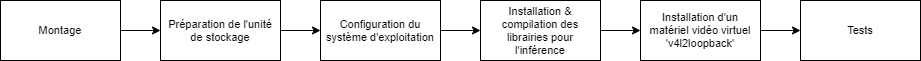
\includegraphics[width=1.0\textwidth]{preparation_nano_ordinateur}
    \caption{Préparation du nano ordinateur}
    \label{fig:preparation_nano_ordinateur}
\end{figure}
\myparagraph{Montage}
\par Le nano ordinateur est une carte mère livrée sans aucun périphérique ni même boitier. Vu que les performances logicielles dépendent des performances matérielles, surtout pour une unité telle qu'un nano ordinateur où les capacités matérielles sont très limitées, la première partie de l'essai a été allouée à la sélection des accessoires et périphériques qui vont permettre d'augmenter les performances, protéger et utiliser confortablement le nano ordinateur. 
\label{montage_nano_ordinateur}
\par L'organigramme de la figure \ref{fig:montage_nano_ordinateur} présente les activités qui composent le montage du nano ordinateur. 
\begin{figure}[H]
    \centering
    
\includegraphics[width=1.0\textwidth]{montage_nano_ordinateur}
    \caption{Montage du nano ordinateur}
    \label{fig:montage_nano_ordinateur}
\end{figure}
\mysubparagraph{Préparation de la carte mère Jetson Nano}
\begin{figure}[H]
    \centering
    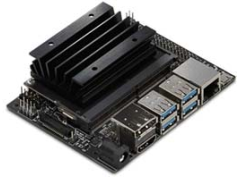
\includegraphics[width=0.5\textwidth]{jetson_nano}
    \caption{Carte mère du nano ordinateur}
    \label{fig:jetson_nano}
\end{figure}
\par Le nano ordinateur qui est livré dans sa boite est uniquement une carte mère, sans unité de stockage, ni boitier, clavier, souris, écran, capacité wifi, ou caméra. Il est uniquement livré avec un câble micro USB qui lui permet d'être démarré avec une alimitation minimale de 5 Volts/2Amp et ne consommer que 5 Watts. Aucun système d'exploitation n'est livré non plus. Vu que de l'objectif de l'essai est de tester les capacités du nano ordinateur et que la consommation sera de plus de 5Watt dues aux branchements de multiples périphériques, certaines "broches" sur la carte mère doivent être activées:  la broche J48 permet de brancher un adaptateur d'alimentation de 5Volts 4Amp au lieu de l'alimentation micro USB; et la broche J38 permet d'activer le PoE (Power-Over-Ethernet) afin d'hériter de l'alimentation du câble Ethernet. Aucune autre préparation sur la carte n'est nécessaire.
\mysubparagraph{Alimentation}
\begin{figure}[H]
    \centering
    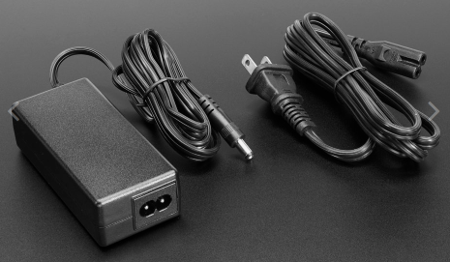
\includegraphics[width=0.5\textwidth]{alimentation}
    \caption{Adaptateur 5 volts 4 amps}
    \label{fig:alimenation}
\end{figure}
\par L'alimentation du nano ordinateur est l'élément matériel le plus important du système. De base le nano ordinateur est livré avec un câble micro USB, lui permettant d'être alimenté en 5Volt 2Amp. Mais le besoin en énergie augmente avec les périphériques qui s'accumulent, tel qu'une caméra. Il est prudent de choisir un adaptateur 5Volt 4Amp d'un fournisseur recommandé par NVIDIA, car un changement de puissance sensible en entrée impacte le fonctionnement opérationnel du nano ordinateur. Deux adaptateurs ont été utilisés, l'un recommandé, et l'autre non, afin de tester leur performance. 
\par Dans le cadre de l'essai, l'alimentation du nano ordinateur est utilisée pour alimenter la carte mère, qui comporte entre autres les CPUs, le GPU, le Hub USB 3.0 interne, le contrôleur Ethernet et le port HDMI. Mais aussi la caméra et  le ventilateur et optionnellement une carte d'extension M.2 NVMe. Afin d'assister l'adaptateur, un hub USB 3.0 externe a été utilisé pour brancher la souris, le clavier, et à un moment donné le dongle Wifi.
\mysubparagraph{Boitier}
\begin{figure}[H]
    \centering
    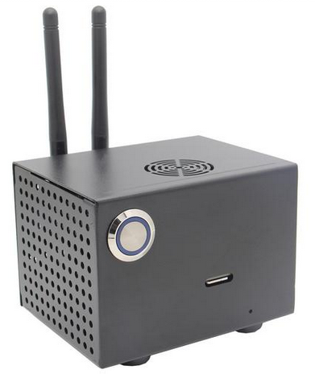
\includegraphics[width=0.45\textwidth]{boitier}
    \caption{Boitier pour le nano ordinateur}
    \label{fig:boitier}
\end{figure}
\begin{figure}[H]
    \centering
    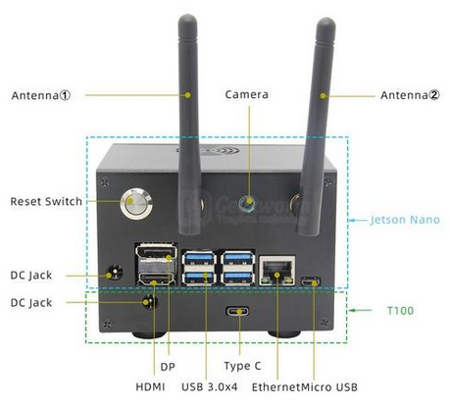
\includegraphics[width=0.5\textwidth]{boitier_back}
    \caption{Vue arrière du boitier pour le nano ordinateur}
    \label{fig:boitier_arriere}
\end{figure}
\par Afin de protéger le nano ordinateur durant l'essai et l'utiliser dans les conditions les plus proches de son futur mode d'opération, il a été installé dans un boitier en métal. Le boitier a été choisi en tenant compte qu'une carte d'extension pour un SSD interne sera installée, ainsi qu'une caméra et un ventilateur. Durant l'essai le nano ordinateur sera manipulé très fréquemment en raison d'un manque d'espace réservé dans la maison. Le boitier permet donc d'éviter de manipuler le matériel et les connecteurs, les protège, évitant de risquer de les briser, et donc ajouter des délais à l'essai. 
\mysubparagraph{Unité de stockage}
\par Le nano ordinateur est conçu pour fonctionner avec un système d'exploitation hébergé sur une carte microSD. Il existe différentes cartes microSD, et certaines sont  beaucoup plus performantes que les autres. Malheureusement les cartes microSD ne sont pas destinées à exécuter un système d'exploitation à temps plein, et leur espérance de vie reste très limitée.  Étant donné que l'objectif du nano ordinateur est d'être en service continuelle à l'extérieure, l'utilisation un disque SSD interne comme alternative semble logique.
\par\underline{Carte microSD}
\par Il existe différentes cartes microSD, de multiples constructeurs, et pour différents usages, mais généralement destiné pour stocker des images et vidéos directement par les appareils multimédias. Leur conception est faite pour la manipulation de gros blocs de données, et non des petits fichiers. Trois cartes microSD 
seront évaluées:
{
    \renewcommand*{\arraystretch}{1.4}
    \begin{table}[ht]
    \centering
    \caption{Cartes microSD}\label{table:cartes_microSD}
    \vspace{0.3em} % Adjust the height of the space between caption and tabular
    \begin{tabular}{l}
        
\includegraphics[width=0.15\textwidth]{micro_sd_evo_plus} microSD Samsung EVO 64Gb Plus XC I Grade 3 Class 10\\
        
\includegraphics[width=0.15\textwidth]{micro_sd_evo} microSD Samsung EVO 64Gb Select XC I Grade 3 Class 10\\
        
\includegraphics[width=0.15\textwidth]{Microsd card Scan Disk Ultra 32Gb class 10 HC I} microSD Scan Disk Ultra 32Gb HC I Class 10\\
    \end{tabular}
    \end{table}
}
{\color{red}\todo{fix le tableau}}
\par\underline{Disque SSD}
% \mysubparagraph{SSD interne Nvme M.2 avec carte d'extension M.2 vers USB3.0}
% \par Pour un appareil destiné à être continuellement en service et à l'extérieure, l'unité de stockage doit être non seulement performante, mais aussi endurante. Un disque SSD interne pour un nano ordinateur est soit une carte d'extension M.2 NVMe ou SATA (selon la carte d'extension), connecté au port PCIe ou USB. Les SSD internes Samsung 970 EVO 250GB NVMe M.2 et Samsung 860 EVO M.2 500GB SATA seront évalués. À noter qu'une carte microSD est tout de même nécessaire pour "bootstrapper" le système d'exploitation. Il n'est pas nécessaire d'avoir une carte microSD performante puisqu'elle n'est utilisée que pour démarrer le système qui se trouve sur le SSD interne. 
\par Un disque SSD et une carte microSD sont différents type de matériel pour différents usages. Le disque SSD est plus adapté pour manipuler les petits fichiers et héberger un système d'exploitation. Il est aussi plus résilient à long terme. C'est donc une option qui ne doit pas être négligée dans le contexte de tests de performance, encore plus avec un nano ordinateur dont les capacités matérielles sont limitées, et qui est un appareil destiné à être continuellement en service et à l'extérieure. L'unité de stockage doit être non seulement performante, mais aussi endurante. Néanmoins, il y a un contreparti important dans la situation d'un nano ordinateur: la consommation d'énergie. Un SSD interne va demander plus d'énergie qu'une carte microSD, et si le nano ordinateur n'est pas capable de gérer correctement les besoins en énergie de ses extensions matériels, le SSD interne risque d'échouer en pleine opération et le nano ordinateur devenir non fonctionnel soudainement.
\par Un disque SSD interne pour un nano ordinateur est soit une carte d'extension M.2 NVMe ou SATA (selon la carte d'extension), connecté au port PCIe ou USB. Les SSD internes Samsung 970 EVO 250GB NVMe M.2 et Samsung 860 EVO M.2 500GB SATA seront évalués.
\begin{figure}[H]
    \centering
    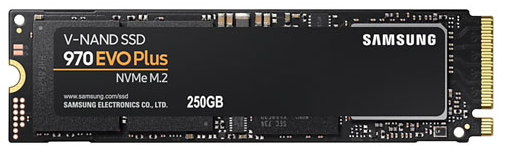
\includegraphics[width=0.5\textwidth]{Samsung 970 EVO Plus 250GB M.2 NVMe Internal Solid State Drive}
    \caption{Disque SSD NVMe M.2 interne 250GB}
    \label{fig:disquessd}
\end{figure}
\par Il y a deux choix qui ont été retenus pendant l'essai pour brancher un SSD interne au nano ordinateur: soit via une carte d'extension M.2 MVMe, et connecté via le Hub USB, soir via une carte d'extension M.2 NVMe connectée au port PCIe interne du nano ordinateur, normalement destinée à une carte d'extension Wifi.
\par Concernant le disque SSD M.2 NVMe connecté à la carte d'extension M.2 via le Hub USB 3.0 interne, le système L4T de NVIDIA ne supporte pas les SSD M.2 NVMe connecté au port USB \footnote{À noter que la carte d'extension T100 est discontinuée et remplacée par la T130}. Il n'est pas reconnu / détecté, il est donc impossible de le formater, de le partitionner, de l'utiliser. Comme il serait risqué pour l'essai de se lancer dans la recompilation du kernel du L4T, une alternative trouvée sur le développeur forum de NVIDIA est de passer par un adaptateur M.2 MVMe connecté au port PCIe interne.
\par Malheureusement cette alternative a rapidement été abandonnée. Il a été possible de démarrer et installer le système d'opération sur le SSD M.2, et faire quelques tests, mais pour une raison inconnue, le système n'était pas stable et devenait non opérationnel assez rapidement, le système perdant la connexion au SSD. La durée la plus longue de stabilité observée a été de moins 30 minutes. Une hypothèse est une baisse d'énergie qui survient à un moment et qui impacte l'alimentation du SSD, chaque volt et milliampère étant important pour la stabilité du nano ordinateur. De plus, le raccordement du câble de la carte d'extension M.2 NVMe PCIe avec le SSD M.2 NVMe est très compliqué et risqué pour le câble lui-même. Une autre limitation importante est que cette solution ne permet pas d'utiliser le boitier, car le SSD M.2 ne rentre pas et ne peut même pas être fixé. 
\par Différentes options pour optimiser l'alimentation ont été explorées: utiliser un HUB USB externe et auto alimenté; brancher un câble Ethernet au lieu d'utiliser un Dongle Wifi; allumer le ventilateur dès le démarrage du nano ordinateur; et l'option de fournir 6Amp directement supportée par la carte mère via les pins; explorer les solutions sur les forums de discussion \footnote{\url{https://www.kingston.com/en/community/articledetail/articleid/48543}} \footnote{\url{https://geekworm.com/products/nvidia-jetson-nano-nvme-m-2-ssd-shield-t100-v1-1}}.
\mysubparagraph{Caméra}
\begin{figure}[H]
    \centering
    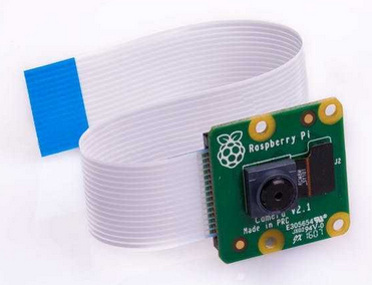
\includegraphics[width=0.40\textwidth]{camera}
    \caption{Caméra}
    \label{fig:camera}
\end{figure}
\par L'objectif du nano ordinateur est d'être utilisé pour détecter continuellement les délimitations de la piste cyclable. Il est évident qu'une caméra doit donc faire partie du système et faire partie de l'évaluation des performances. Néanmoins, durant le déroulement de l'essai, la caméra sera très peu utilisée. En effet il n'est pas évident d'être dans un mode de développement directement sur le terrain. Un matériel vidéo virtuel sera utilisé pour simuler la caméra et alimenter l'inférence avec des vidéos préenregistrées, permettant ainsi d'évaluer les performances de l'inférence avec des vidéos, même si d'un point de vue performance matérielle l'utilisation ne sera pas équivalente. Les performances matérielles de l'inférence en temps réel seront évaluées avec la caméra, même si la vue de la caméra n'est pas la piste cyclable, ce qui n'est pas important pour ce test, peu importe ce qui est détecté. 
\par la caméra qui a été sélectionnée est la version 2 de celle du fournisseur Raspberry Pi, le concurrent directe du nano ordinateur NVIDIA Jetson Nano. Cette caméra a été épprouvée avec le temps, est performante, elle semble être la plus adaptée pour ce genre de projet. 
\mysubparagraph{Ventilateur}
\begin{figure}[H]
    \centering
    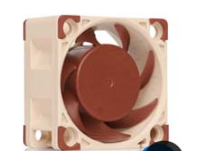
\includegraphics[width=0.35\textwidth]{fan}
    \caption{Ventilateur}
    \label{fig:fan}
\end{figure}
\par Un système informatique a besoin d'un ventilateur pour évacuer la chaleur produite par ses processeurs et les autres éléments électroniques, et éviter une faute opérationnelle et des bris de matériel. L'objectif du nano ordinateur étant d'être opérationnel continuellement, et ses éléments étant contenus dans un boitier, il est encore plus indispensable d'installer un ventilateur. Le ventilateur choisi a pu être installé dans le boitier, même si le boitier ne possède de support pour le fixer. Le ventilateur est capable de démarrer automatiquement au besoin, mais il est volontairement démarré manuellement dès que le nano ordinateur est démarré. Cela évite que la chaleur ne s'accumule, qu'elle soit tout de suite ventilée à l'extérieure, évitant un risque de surchauffe, la capacité du ventilateur étant tout de même limité (petit modèle).
\mysubparagraph{Hub USB externe 3.0 4 ports}
\begin{figure}[H]
    \centering
    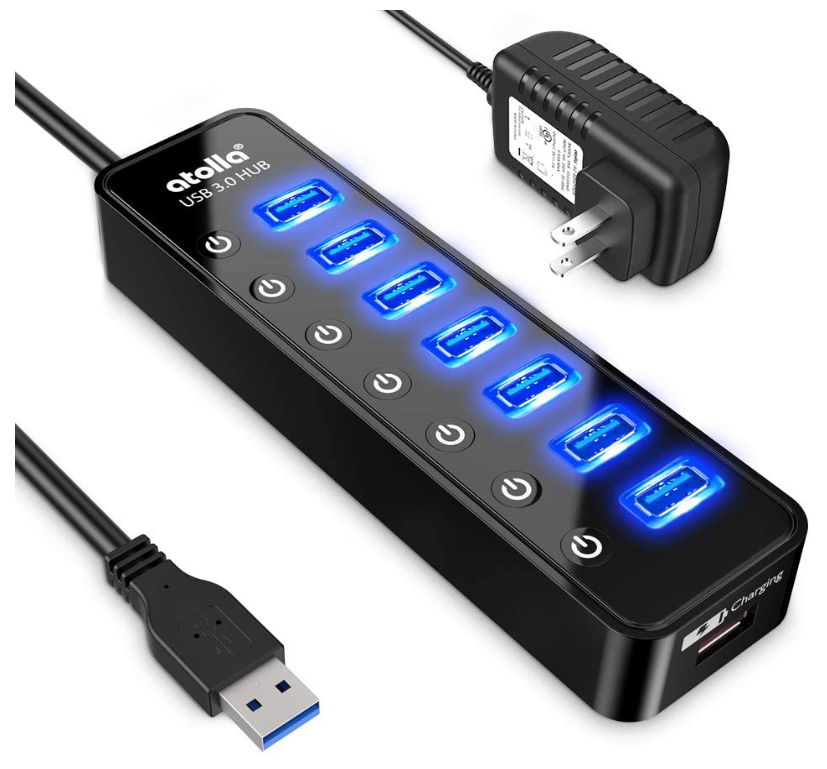
\includegraphics[width=0.4\textwidth]{Powered USB Hub 3.0, Atolla 7-Port USB Data Hub Splitter with One Smart Charging}
    \caption{Hub USB 3.0 externe autoalimenté}
    \label{fig:hubusb}
\end{figure}
\par Le nano ordinateur comprend un hub USB 3.0 4 ports internes, les 4 ports étant connectées via le même contrôleur. Ce hub consomme de l'énergie pour alimenter les périphériques qui y sont connectés, comme un SSD interne ou un dongle Wifi, et gérer l’ échange de données. Afin de minimiser les besoins en alimentation et optimiser le plus possible le transfert de données, la souris, le clavier et le dongle USB ont été branchés a un hub USB 3.0 externe autoalimenté. Malheureusement cette option complexifie le déploiement sur le terrain du nano ordinateur. L'alternative pour s'en passer est d'utiliser un câble Ethernet, PoE préférablement, à la place d'un dongle Wifi qui est très gourmant en termes de besoin en alimentation, et chauffe rapidement.
\mysubparagraph{Réseau Internet}
\par Le nano ordinateur comprend un contrôleur Ethernet pour brancher un câble réseau et se brancher sur Internet. Selon la configuration de la carte mère, le nano ordinateur peut hériter de l'alimentation via Ethernet (PoE), via la broche J38. Il comprend aussi un port PCIe interne qui permet de brancher une carte d'extension Wifi. L'autre alternative étant de passer par un dongle USB Wifi, ou un périphérique Wifi externe connecté au port USB. 
\par Dans le cadre de cet essai, le périphérique Wifi externe USB a été utilisé en premier puisque déjà disponible. Malheureusement les performances étaient assez décevantes, le réseau Wifi à la maison n'étant pas non plus très performant dans la pièce ou le nano ordinateur était installé (table de la cuisine). Un débit d'environs 5Mbits était disponible. Par curiosité un dongle USB Wifi a été acquis, mais autant décevant. La meilleure alternative pour améliorer le déroulement de l'essai a été de tirer un câble Ethernet et d'installer un router secondaire, et de brancher le nano ordinateur a ce nouveau router. L'accès Internet a été plus stable et de bien meilleure qualité, la connexion étant d'environs 11Mbs. 
\par Le PoE n'a pas été évalué. 
\myparagraph{Préparation de l'unité de stockage}
Le nano ordinateur est conçu pour fonctionner avec une microSD, et NVIDIA fournit uniquement de la documentation à cet effet. L'option d'utiliser un disque SSD interne est disponible sur Internet, mais n'est pas supporté officiellement par NVIDIA. Il existe néanmoins des articles à ce sujet dans le forum des développeurs\footnote{\url{https://forums.developer.nvidia.com/t/how-to-connect-ssd-to-jetson-nano/74053}}. 
\mysubparagraph{Carte microSD}
\par NVIDIA fournit de la documentation très claire et simple afin de préparer la carte microSD (formattage) et installer l'image du JetPack.\footnote{\url{https://developer.nvidia.com/embedded/learn/get-started-jetson-nano-devkit#write}}.
\mysubparagraph{Disque SSD}
\par La procédure d'installation pour installer JetPack sur le SSD interne est disponible sur le site "jetsonhacks.com"\footnote{\url{https://www.jetsonhacks.com/2019/09/17/jetson-nano-run-from-usb-drive/}}. À noter qu'une carte microSD est tout de même nécessaire pour "bootstrapper" le système d'exploitation. Il n'est pas nécessaire d'avoir une carte microSD performante puisqu'elle n'est utilisée que pour démarrer le système qui se trouve sur le SSD interne. 
\myparagraph{Configuration du système d'exploitation}
\par La première fois que le système démarre, le système Ubuntu Linux For Tegra (L4T) doit être configuré avec toutes les options personnalisées (langue, clavier, timezone, etc.).
\myparagraph{Installation \& compilation des librairies pour l'inférence}
\par Les librairies pour la segmentation sémantique 
d'images et de vidéos via l'inférence de modèles déjà préparée sont mises à disposition par NVIDIA via un projet dans GitHub. La documentation pour l'installation et l'inférence est disponible directement dans la page GitHub. 
\myparagraph{Installation d'un matériel vidéo virtuel 'v4l2loopback'}
\par L'inférence fournie par NVIDIA est conçue pour utiliser la caméra du nano ordinateur. Ce qui n'est pas forcément "pratique" pour évaluer la segmentation sémantique d'une vidéo d'une piste cyclable. Heureusement un matériel vidéo virtuel permet de simuler la caméra et d'alimenter l'inférence avec une vidéo enregistrée, au lieu de la caméra. La contrepartie concerne l'évaluation des performances:  en effet la caméra demande plus de puissance au nano ordinateur que le simulateur logiciel.
\myparagraph{Tests}
\par Afin de s'assurer que le nano ordinateur est prêt pour être évalué, des tests matériels et logiciels sont  effectués une fois le système monté et stabilisé. Les résultats des tests servent de référence pour évaluer l'état de santé du nano ordinateur. 
\subsubsection{Collecte des données}
\par 
\vspace{1\baselineskip}
\par \label{section:collecte_donnees}
\subsubsection{Mise en place des solutions logicielles}
\myparagraph{Jetson Nano}
\vspace{0.5\baselineskip}
\\
\noindent Le nano-ordinateur est destiné à l'inférence. NVIDIA fournit tout un système d'installation, qui est nommé JetPack, et qui contient un système d'exploitation basée sur Ubuntu, "\acrlong{l4t}" \acrshort{l4t}), la plateforme applicative et les librairies nécessaires pour l'inférence, tels que Python, pytorch, les modèles préentrainés au format \acrshort{onnx}, le compilateur CUDA, et le \acrshort{sdk} TensorRT.
\myparagraph{Calcul Québec}
\vspace{0.5\baselineskip}
\\
\noindent Le nano-ordinateur est destiné à l'inférence, et non l'entrainement d'architectures. Il n'est pas non plus destiné à être un environnement de développement. Un autre environnement de travail est donc nécessaire pour développer, et doit posséder les capacités matérielles (\acrshort{gpu}s, mémoires, espace de stockage) et logicielles (librairies) pour entrainer une architecture. Le professeur Mickaël Germain, directeur de projet, m'a présenté l'environnement de Calcul Québec. Celui-çi fournit un espace de travail scientifiques destiné aux chercheurs et aux universitaires, qui m'a permit  de pouvoir travailler avec l'apprentissage profond, compiler un fork de torchvision, réentrainer des architetures, générer les versions \acrshort{onnx}, et ainsi contourner les limitations du nano-ordinateur. Avoir accès à cet environnement de travail a été un élément clé dans le cadre de cet essai.
\mysubparagraph{Compte Calcul Québec}
\vspace{0.5\baselineskip}
\\
\noindent Calcul Québec mets à disposition des ressources matérielles puissantes et l'accès a des libraires de haute technologie telle que pour l'apprentissage profond, permettant d'avoir un environnement de travail professionnel et performant rapidement. Les ressources matérielles à disposition sont des grappes de serveurs, de \acrshort{cpu}s et \acrshort{gpu}s de différents types, ainsi que de l'espace de stockage. Les librairies sont disponibles via un repository privé, et lorsque certaines étaient manquantes (\acrshort{onnx} et onnxruntime), j'ai fait une demande par courriel. L'administrateur a pu rendre disponible l'une des deux (\acrshort{onnx}), la seconde (onnxruntime) étant beaucoup plus complexe a installé, pour l'avoir tenté sur le nano-ordinateur. 
\vspace{0.5\baselineskip}
\\
\noindent L'autre avantage de l'environnement de Calcul Québec est la mise à disposition de Jupyter Notebook, afin de tester rapidement du code Python. Par contre il n'est pas conseillé d'exécuter du code nécessitant des délais, tels que l'entrainement d'une architecture. 
\vspace{0.5\baselineskip}
\\
\noindent L'un des irritants est de ne pas pouvoir exécuter un conteneur Docker tel quel. Il faut le convertir au format Singularity. Dans le cadre du projet cela m'aurait facilité la tâche, car NVIDIA fournit des conteneurs Docker prêts à l'utilisation pour le réentrainement. Je n'ai malheureusement pas pris le temps et la chance de convertir un conteneur Docker au format Singularity. Je ne sains pas si c'est une activité assez simple ou complexe, mais du peu que j'ai lu cela semble assez "rapide".
\mysubparagraph{Jupyter Notebook}
\vspace{0.5\baselineskip}
\\
\noindent Le besoin de tester du code Python est toujours nécessaire. La console Python n'étant vraiment pas conviviale, un environnement Jupyter Notebook est un compromis incontournable. Heureusement Calcul Québec fournit un accès à des notebooks depuis Internet, permettant en plus d'hériter de leur environnement de travail. Il est à noter que les notebooks n'ont pas été utilisés pour entrainer une architecture ou générer les versions \acrshort{onnx}, mais de tester du code Python simple, comme visualiser des images, transformer des tensors, et évaluer la segmentation prédite générée avec le vérité terrain (\acrshort{gt}). 
\paragraph{NVIDIA}
\mysubparagraph{Compte NVIDIA}
\vspace{0.5\baselineskip}
\\
\noindent NVIDIA mets à disposition tout un écosystème éducatif permettant aux développeurs et aux chercheurs d'obtenir de l'aide au sujet de leur produit et librairies. Dans le cadre de l'essai, un compte NVIDIA a été créé, permettant d'accéder au forum de développeurs, et les conterneurs Docker par exemple. Il est aussi possible d'accéder à du matériel éducatif grâce à l'institut DeepLearning de NVIDIA, dont l'accès a été commandité par le professeur Mickaël Germain, directeur de projet. Le forum de développeurs a été un outil utile dans le cadre de ce projet, car le dépôt d'une question m'a permis de me débloquer. Je n'étais pas capable de regénérer la version \acrshort{onnx} à partir du code source et de la documentation fournie par NVIDIA pour une architecture \acrshort{fcn}. Le développeur principal de l'application a répondu et m'a guidé dans la résolution du problème. Les autres ressources ont eu un impact limité dans le cadre de ce projet, puisque par exemple le conteneur Docker et DIGITS n'ont pas pu être utilisé. Le code source des architectures est disponible sans nécessiter de compte, de même que les \acrshort{sdk}s Jetpack.
\mysubparagraph{NVIDIA DIGITS}
\vspace{0.5\baselineskip}
\\
\noindent NVIDIA fournit aux développeurs un environnement visuel permettant de réentrainer les architectures \acrshort{fcn} qu'ils fournissent avec leurs propres dataset. Cet environnement se nomme DIGITS. Malheureusement il est nécessaire d'avoir son propre matériel, le système d'exploitation Ubuntu 18.04 LTS, d'avoir au moins un \acrshort{gpu}. DIGITS ne s'installe pas sur le nano-ordinateur, ni sous Windows, ni avec la version "\acrshort{wsl}" (\acrlong{wsl}). Cette option a donc été abandonnée rapidement. 
\mysubparagraph{Conteneur Docker NVIDIA}
\vspace{0.5\baselineskip}
\\
\noindent NVIDIA fournit aux développeurs des conteneurs Docker, avec tout ce qui est nécessaire pour réentrainer une architecture et regénérer une version \acrshort{onnx}, par exemple. Malheureusement la capacité du nano-ordinateur ne permet pas de travailler efficacement avec un conteneur Docker, le nano-ordinateur devient sans réponse, nécessitant un redémarrage forcé. Cette option a donc été aussi abandonnée rapidement. 
\mysubparagraph{NVIDIA DeepStream}
\vspace{0.5\baselineskip}
\\
\noindent Durant le déroulement de l'essai, NVIDIA a mis à disposition un environnement d'apprentissage profond, nommé "DeepStream", facilitant la conception et la génération de modèles, jusqu'à l'inférence. Cet outil n'a pas été évalué, mais pourrait être un outil alternatif pour réentrainer une architecture.
\subsection{Évaluation}
\label{metho_eval}
\begin{figure}[H]
    \centering
    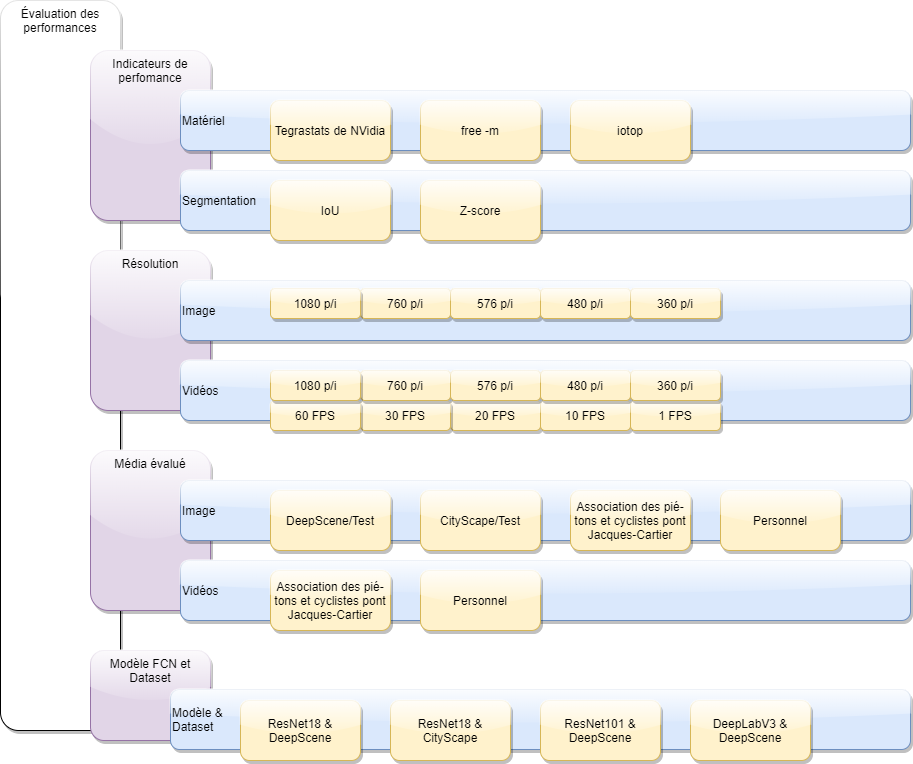
\includegraphics[width=1.0\textwidth]{metho_eval_perf_round_glass_shadow}
    \caption{Éléments pour l'évaluation des performances}
    \label{fig:metho_eval}
\end{figure}
\subsubsection{Stratégie de test}
\par L'objectif principal de l'essai est de déterminer la capacité et les limites du nano ordinateur d'inférer en temps réel des modèles de réseau de neurones à convolution entier pour la segmentation sémantique de vidéos. La stratégie qui sera appliquée sera de tester avec divers modèles et divers niveaux de qualité vidéos, en espérant trouver le compromis qui répond le mieux à cet objectif.
\begin{enumerate}
   \item \label{metho:testbaseinférence} Afin de s'assurer du bon fonctionnement du nano ordinateur et d'avoir des résultats de référence propre à notre environnement, l'inférence sera testée avec des modèles existants et pré entrainés pour la segmentation sémantique, avec les images et les vidéos provenant des références, et dont les caractéristiques et les résultats sont disponibles. 
   \item \label{metho:testbaseinférencesite} En espérant que les tests de l'étape \#\ref{metho:testbaseinférence} précédente donnent les résultats documentés dans les articles de références, ils seront repris avec les mêmes modèles, mais avec les images et les vidéos du site d'étude possédant la meilleure qualité acquise (1080p/i, 30FPS). Les données sources (images et vidéos) devront subir certains prétraitements à ce effet, afin de répondre aux requis des modèles.
   \item \label{metho:testdevinférencesite} Selon les résultats de l'étape \#\ref{metho:testbaseinférencesite}, les tests se concentreront sur l'inférence avec des vidéos, en réduisant progressivement la résolution (760p/i, 576p/i, 480p/i, 360p/i) et le nombre d'images par seconde (20FPS, 10FSP, 1FPS).
   \item Les étapes intermédiaires de l'étape \#\ref{metho:testdevinférencesite} précédente seront de 1) valider les résultats de l'inférence avec des images avant de tester avec les vidéos, et 2) évaluer si les modèles de réseaux de neurones à convolution entiers doivent et/ou peuvent être adaptés facilement, en tenant compte de l'échéancier de l'essai, et ce afin de répondre à l'objectif principal.
\end{enumerate}
\subsubsection{Stratégie de collecte des indicateurs de performance}
\par La méthodologie de la collecte des indicateurs est la suivante\footnote{\url{https://vince7lf.github.io/2020/05/26/metrics.html}}: 
\begin{itemize}    
    \item La collecte est démarrée après un démarrage frais, manuellement, via un script shell, qui exécute chaque outil, et attend l'interruption du test. 
    \item Chaque outil qui est utilisé pour collecter les mesures, possède son propre fichier.
    \item La date et l'heure de chaque indicateur collecté sont précisées.
    \item Afin de faciliter la documentation et l'analyse du test, des points d'intérêt sont ajoutés dans un fichier séparé pour marquer un moment particulier du test, avec la date, l'heure et un libellé. Ce point d'intérêt est fait grâce à une commande "shell" qui vient ajouter une trace dans ce fichier.
    \item Chaque indicateur est collecté toutes les secondes.  
    \item Une fois le test complété, la collecte est arrêté manuellement. 
    \item Chaque fichier est ensuite transformé en fichier CSV, via des commandes shell.
    \item À partir des fichiers CSV un script Python génère les graphiques automatiquement. 
\end{itemize}
\par Chaque indicateur est une colonne du fichier CSV. Il existe le même nombre d'indicateurs à tout moment. La date et l'heure sont un champ. 
\par Avant tout début de tests, la collecte est démarrée sans activité autre que la collecte des indicateurs. Cela permet de prendre une base de référence sans aucune charge.
\par Ensuite les tests débutent. 
\par Les indicateurs collectés permettent de créer des graphiques qui montrent la progression de chacun.
\par Les performances matérielles du Jetson Nano sont évaluées grâce à différentes commandes : "tegrastats" fournis par NVIDIA, "free -m" et "iotop".
\par Les performances de la segmentation sont évaluées grâce au IoU et au z-score pour la classe du chemin / route. Une fonction Python est utilisée. Les fonctions IoU et le z-score utilisent l'image prédite (généré par le modèle FCN) et l'image vérité terrain ("ground truth"). Les images originales sont donc présélectionnées selon leur intérêt et l'image vérité terrain ("ground truth") créée. L'image prédite et vérité terrain ("ground truth") doivent utiliser la même palette de couleurs et doivent être de la même résolution. Pour les images qui ne possèdent pas d'image vérité terrain ("ground truth"), cell-ci est créée à la main avec l'éditeur "Gimp". Comme la résolution de la segmentation de l'image prédite par le modèle de NVIDIA est très faible ("carrée"), l'image vérité terrain ("ground truth") ne sera pas précise au pixel prêt. Le besoin est d'évaluer et non d'entrainer, l'importance de la précision de la classification est moindre dans ce cas. 
\subsubsection{Segmentation avec des images}
\myparagraph{Préparation et post-traitement}
\vspace{\baselineskip}
\\
\noindent Afin de pouvoir mesurer les performances de la segmentation (IoU, F1 score), les classes et la palette de couleur entre l'image vérité terrain (\acrshort{gt}) et celles prédites doivent être les mêmes.
\vspace{\baselineskip}
\\
\noindent L'image vérité terrain (\acrshort{gt}) du jeu de donnée original DeepScene ne possède pas la même palette de couleur ni exactement les mêmes classes que celle de l'architecture.
\vspace{\baselineskip}
\\
\noindent Un travail d'uniformisation est nécessaire avant la segmentation, qui est résumée dans le tableau \ref{table:classes_palette_couleur}.
{
    \renewcommand*{\arraystretch}{1.4}
    \begin{table}[h]
    \centering
    \caption{Classes et palettes de couleur}\label{table:classes_palette_couleur}
    \vspace{0.1em} % Adjust the height of the space between caption and tabular
    \begin{tabular}{{@{}|p{4em}|p{6em}||p{4em}|p{6em}||p{4em}|p{6em}|@{}}}
        \hline
        \multicolumn{2}{|c||}{\textbf{DeepScene}} & \multicolumn{2}{c||}{\textbf{NVIDIA}} & \multicolumn{2}{c|}{\textbf{Consolidée}} \\
        \hline
        \multicolumn{1}{|l|}{\textbf{Classes}} & \multicolumn{1}{c||}{\textbf{RGB}} & \multicolumn{1}{l|}{\textbf{Classes}} & \multicolumn{1}{c||}{\textbf{RGB}} & \multicolumn{1}{l|}{\textbf{Classes}} & \multicolumn{1}{c|}{\textbf{RGB}} \\
        % \thead{Classes \\ DeepScene} & \thead{RGB \\ DeepScene} & \thead{Classes \\ NVIDIA} & \thead{RGB \\ NVIDIA} & \thead{Classes \\ consolidées} & \thead{RGB \\ consolidées} \\
        \hline
        \hline
        Road & 170-170-170 & Trail & 200-155-75 & Trail & \textcolor{red}{170-170-170}\\
        \hline
        Grass & 0-255-0 & Grass & 85-210-100 & Grass & \textcolor{red}{0-255-0}\\
        \hline
        Vegetation & 102-102-51 & Vegetation & 15-100-20 & Vegetation & \textcolor{red}{102-102-51}\\
        \hline
        Tree & 0-60-0 & - & - & \textcolor{red}{Vegetation} & \textcolor{red}{102-102-51}\\
        \hline
        Sky & 0-120-255 & Sky & 0-120-255 & Sky & 0-120-255\\
        \hline
        Obstacle & 0-0-0 & Obstacle & 255-185-0 & Obstacle & \textcolor{red}{0-0-0}\\
        \hline
    \end{tabular}
    \end{table}
\vspace{\baselineskip}
\\
\noindent De plus, l'image segmentée prédite par l'architecture ne possède pas précisément la même palette de couleur que celle qui est configurée, il y a quelques différences minimes dans les codes couleurs RGB (par exemple 0-119-255 au lieu de 0-120-255), mais qui doivent être arrangée afin de pouvoir être correctement évaluées. 
\vspace{\baselineskip}
\\
\noindent Un travail de traitement de l'image segmentée prédite est nécessaire avant l'évaluation de la segmentation.
\myparagraph{Segmentation et évaluation}
\vspace{\baselineskip}
\\
\noindent Afin de tester la performance de la segmentation du modèle, deux images du jeu de données de DeepScene sont utilisées, car ce jeu contient déjà les images vérités terrain (\acrshort{gt}), un gain de temps non négligeable dans le cadre de l'essai. Uniquemement la classe "Trail" est évaluée.
\vspace{\baselineskip}
\\
\noindent L'architecture fournit à l'utilitaire "segnet-console" est "fcn-resnet18-deepscene-576x320" \footnote{\url{segnet-console -{}-network=fcn-resnet18-deepscene -{}-visualize=mask -{}-alpha=10000 images/city_0.jpg output.jp}}. 
\vspace{\baselineskip}
\\
\noindent Un script Python\footnote{\url{https://gist.github.com/ilmonteux/8340df952722f3a1030a7d937e701b5a}} est utilisé afin de mesurer le \acrshort{iou} et le F1 score de la classe de l'image prédite par l'architecture.
\subsubsection{Segmentation avec des vidéos}
\myparagraph{Préparation et pré-traitement}
\par L'évaluation de la segmentation avec des vidéos va s'effectuer non pas avec la caméra, mais avec un matériel vidéo virtuel. En effet, il n'est pas réaliste de pouvoir travailler sur le terrain. La commande "segnet-camera" permet de fournir en option le matériel qui doit être utilisé, par exemple "/dev/video0" pour la caméra. Le module "v4l2loopback"\footnote{\url{https://github.com/umlaeute/v4l2loopback}} permet de créer un matériel vidéo virtuel "/dev/video1". Ce matériel permet de recevoir un flux vidéo, qui pourra alors alimenter l'utilitaire "segnet-camera", comme le ferait la caméra. Le flux vidéo sera produit par l'utilitaire "gstreamer" avec comme données d'entrées le fichier de la vidéo et dirigé vers le matériel vidéo virtuel "/dev/video1".
\par La difficulté réside dans le fait que le matériel vidéo virtuel et le flux vidéo doivent être compatibles avec ce que l'utilitaire "segnet-camera" s'attend, et qui a été conçu pour être compatible avec une caméra. 
\par Le diagramme de la figure \ref{fig:arch_segmentation_video} résume à haut niveau les relations entre ces éléments. Pour comparaison, le diagramme de la figure \ref{fig:arch_segmentation_camera} montre la segmentation avec la caméra. 
\begin{figure}[H]
    \centering
    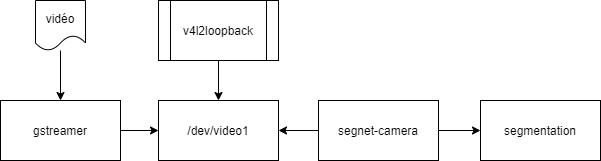
\includegraphics[width=.5\textwidth]{arch_segmentation_video}
    \caption[Diagramme d'architecture de la segmentation d'une vidéo]{Diagramme d'architecture de la segmentation d'une vidéo}
    \label{fig:arch_segmentation_video}
\end{figure}
\begin{figure}[H]
    \centering
    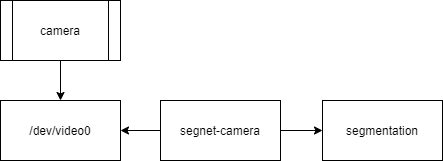
\includegraphics[width=.5\textwidth]{arch_segmentation_camera}
    \caption[Diagramme d'architecture de la segmentation avec la caméra]{Diagramme d'architecture de la segmentation avec la caméra}
    \label{fig:arch_segmentation_camera}
\end{figure}
\myparagraph{Segmentation et évaluation}
\par Les tests de performance de la segmentation de vidéos se déroulent de la manière précisée dans la section "\ref{section:strategie_test_inference} \nameref{section:strategie_test_inference}". 
\par L'un des avantages de l'utilitaire "gstreamer" est de pouvoir contrôler la résolution et le nombre d'images par seconde (\acrshort{fps}) de la vidéo qui doit être segmentée. Les différentes résolutions et \acrshort{fps} qui désirent être exécutées sont préparées dans un script "shell" écrit pour l'occasion. Le script s'occupe de démarrer gstreamer avec les bons paramètres, et en parallèle de démarrer la segmentation avec "segnet-camera". Un jeu de résolution peut être testé unitairement\footnote{\url{https://github.com/vince7lf/gae724/blob/master/run_deepscene.sh}}, ou plusieurs en séquence\footnote{\url{https://github.com/vince7lf/gae724/blob/master/run_deepscene_batch.sh}}. 
\par Les résolutions et images par seconde qui ont été testées sont résumées dans le tableau "\ref{table:resolutions_tested}". 
\par Deux vidéos ont été utilisées pour tester la segmentation. La première vidéo est utilisée pour tester l'inférence avec une vidéo du site d'étude, et qui a été fournie gracieusement par l'\acrlong{apcpontjc}. Cette première vidéo est intéressante, car elle est filmée en mouvement par un cycliste. Dans un interval de 30 secondes, l'angle de vue change rapidement. La piste cyclable est bordée d'un muret côté sud, et de la route avec les voitures qui circulent côté nord. Même si la journée est ensoleillée, la surface de la piste est aussi à un moment humide.
\par La seconde vidéo est utilisée pour tester la segmentation avec les différentes résolutions et images par seconde. C'est une vidéo d'une petite piste cyclable qui est dans mon quartier, et que j'ai prise en marchant avec mon téléphone intelligent. La vidéo est intéressante, car dans un interval de 30 secondes l'état de la piste passe d'une scène ensoleillée à ombragée, sèche à mi-sèche, avec un petit ou gros banc de neige en bordure, ou qui s'aventure un peu sur la piste, bordée d'herbe mouillée ou sèche.
\subsection{Adaptation}
\noindent La phase d'adaptation sera initiée si le temps le permet, et s'il est jugé bon d'améliorer la qualité de la segmentation. Il y a deux types d'adaptation possible: matérielle et logicielle.
\vspace{\baselineskip}
\\
\noindent L'adaptation matérielle sera jugée nécessaire si le nano ordinateur ne peut être utilisé tel quel pour répondre aux objectifs. Par exemple si le nano ordinateur devient non utilisable (lent ou sans réponse) après un certain temps. La stratégie sera de diagnostiquer le comportement et d'évaluer un remède. L'une des pistes de solution privilégiée sera de lui apporter plus de puissance, comme de l'ajout de mémoires ou un espace de stockage plus performant. Plus complexe, optimiser le processus, par exemple certains traitements, serait aussi une option.
\vspace{\baselineskip}
\\
\noindent L'adaptation logicielle, quant à elle, sera jugée nécessaire si la prédiction de la segmentation est en deçà des attentes, ou inutilisable. Le choix d'adapter un modèle avec les méthodes de "Transfer Learning" et "Domain adaptation" sera la première option privilégiée, car cela procure un gain de temps non négligeable: il n'y a pas besoin de passer à travers tout le processus "essai-erreur", couteux en temps, en énergie et en ressources matérielles, d'apprentissage et de paramétrisation du modèle. Des efforts conséquents seront par contre nécessaires pour générer les images vérités terrain \acrshort{gt} avec le jeu de données local, celui de l'\acrshort{apcpontjc} de préférence, personnel ou autre sinon.
\vspace{\baselineskip}
\\
\noindent Le diagramme de la figure \ref{fig:metho_adaptation} présente la méthodologie qu'il faut suivre pour adapter un modèle à un nouveau jeu de données et à une autre résolution. La première étape est de sélectionner un modèle déjà entrainé et qui semble pouvoir être le meilleur candidat pour aider à répondre à la problématique. C'est un travail de recherche et de test minutieux, qui est le plus important de toutes les étapes. La seconde activité est conséquente en efforts: préparer le jeu de données, incluant les images vérité terrain, les bonnes résolutions, déterminer les classes et la palette de couleurs nécessaires. L'étape suivante est d'étudier l'architecture du modèle, afin de l'adapter au jeu de données, aux classes, et au besoin modifier les couches de l'architecture afin d'avoir une segmentation la plus précise et fine possible. Une fois ces étapes de préparation complétées, le ré entrainement du modèle peut s'effectuer, et la segmentation évaluée. Cette phase d'adaptation est un processus itératif, qui peut être représenté par la figure \ref{fig:methodologie_complexe_realiste}.
\label{metho_adaptation}
\begin{figure}[H]
    \centering
    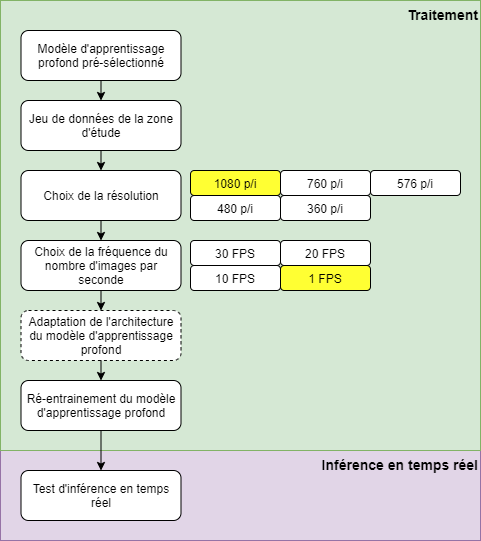
\includegraphics[width=0.65\textwidth]{metho_traitement_eval.png}
    \caption{Méthodologie du traitement et adaptation}
    \label{fig:metho_adaptation}
\end{figure}
\subsubsection{Choix du modèle de l'architecture FCN}
\noindent Le premier modèle qui est évalué est celui de l'architecture SegNet18 entrainée avec le jeu de données "DeepSCene", et fourni par NVIDIA. Le second de la liste, et qui est aussi déjà fourni par NVIDIA, est l'architecture de SegNet18 entrainée avec le jeu de donnée "CityScape". Les deux autres architectures, ResNet101 \& DeepScene et DeepLabV3 \& Deepscene, ne sont pas disponibles et devront être préparées et entrainées, mais elles sont attrayantes du point de vue de leur réputation et de leur potentiel, et vouloir les adapter au contexte de l'essai semble logique. Une dernière boite vide est disponible, afin de laisser une porte ouverte à une potentielle opportunité d'entrainer une architecture tout à fait personnalisée, par exemple une adaptation de l'architecture de DeepLabV3 avec le jeu de données de l'\acrshort{apcpontjc}.\label{section:choix_modele_architecture}
% \subsubsection{Adaptation du modèle}
% % {\color{red}\todo{TODO}}
% \subsubsection{Ré-entrainement du modèle}
% % {\color{red}\todo{TODO}}

\section{Résultats -- 10-15 pages}
\par Voici le plan qui est utilisé pour rédiger les résultats.
\begin{itemize}
   \item \label{resultat1}Pour chaque modèle et résolution utilisés, la segmentation sémantique de certaines images et vidéos sera présentée. La segmentation qui a réussi, celle qui est moins précise, et celle qui a échoué seront soulignées. Un résumé du \% de succès vs des échecs sera fait, selon les modèles et les résolutions. 
   \item En complément de la section précédente, les performances du Jetson nano pour les divers scénarios de test seront résumés avec différents indicateurs. Ceux qui ont échoué ou n'ont pas été possibles en raison des limitations du nano-ordinateur seront indiqués. 
   \item Enfin les performances de l'inférence et des modèles de réseaux de neurones pour la segmentation sémantique seront listées. Des indicateurs de performance classiques et tirés de la littérature seront utilisés.
\end{itemize}

\section{Interprétation et discussion des résultats -- 5-7 pages}
\subsection{Performances matérielles}
\subsubsection{Stockage de données}
\par Les tests montrent que le \acrshort{ssd} interne est de 4 à 11 fois plus efficaces qu'une carte microSD, pour l'opération de lecture de données. 
\subsubsection{Performances système}
\myparagraph{Performances globales}
\par Concernant les performances globales du nano ordinateur, il est à noter que celui-ci est capable d'exécuter l'inférence en temps réel pour une durée prolongée (23 minutes dans ce cas), et rester réactif aux commandes. L'exemple qui le démontre est le démarrage du navigateur Chromium entre deux segmentations, et pendant la segmentation.
\myparagraph{Fréquence}
\par La commande "tegrastats" offre la fréquence des \acrshort{cpu}s (4 pour le nano ordinateur), le GR3D (\acrshort{gpu}) et EMC. On peut noter que l'inférence prend 100\% du GR3D pendant toute la durée. Les \acrshort{cpu}s sont tous utilisés équitablement pendant l'inférence, en dépassant rarement les 30\% d'utilisation. En fait la période qui montre une exploitation élevée des \acrshort{cpu}s est lors de l'utilisation de Chromium, ou l'ensemble des \acrshort{cpu}s sont employés entre 0\% et 90\%. 
\par Il faut donc rester vigilant quand à l'utilisation des \acrshort{cpu}s pendant l'inférence sur le long terme, au risque de perdre le système en raison d'un ralentissement progressif dû à un manque de ressources processeurs \acrshort{cpu}s.
\myparagraph{Mémoire}
\par La commande "free -m" offre l'utilisation mémoire du système en Mb. Le nano ordinateur au démarrage ne consomme qu'environ 1.5Gb de mémoire totale, et possède 4Gb de libres sur un total de 6 Gb(d'où proviennent les 6Gb du graphique ?\todo{TODO}). À la fin du test de 25 minutes, il ne reste qu'environs 3Gb de mémoire libre, un peu plus de 2Gb semble resté utilisé. De la mémoire swap a commencée à être consommée lors du démarrage de Chromium pendant la 3e segmentation, et ne semble jamais avoir été libérée. La mémoire tampon cachée est aussi sensiblement utilisée et revient un peu en dessous de son niveau original à la fin du test. 
\par De même que pour l'utilisation des processeurs, il semble être préférable de rester vigilant lors de l'utilisation opérationnelle du nano ordinateur, la segmentation consommant de la mémoire qui semble ne plus être disponible pour les autres ressources du système, comme le démontre l'état de la mémoire totale libre à la suite de l'arrêt de la 1re segmentation. 
\myparagraph{I/O}
\par La commande "iotop" offre les performances I/O du nano ordinateur pendant le test de 25 minutes. Le I/O de la segmentation est très raisonnable, de même que celle du système. Il n'y a quasiment pas d'opération visible en écriture, même la collecte des statistiques durant le test, aux secondes, n'apparait pas. Les opérations en lecture sont plus visibles, mais très ponctuelles. La période la plus occupée en lecture semble être due durant le démarrage de la segmentation la première fois: le système semble lire le modèle en mémoire, et le conserver en mémoire, car les opérations en lecture suivantes sont peu ou non visibles pendant le démarrage des segmentations suivantes.
\par Cela expliquerait l'augmentation de l'utilisation de la mémoire à la suite de la segmentation. 
\myparagraph{Température}
\par La commande "tegrastats" offre grâce à des capteurs intégrés à la carte mère la température de différents éléments matériels du nano ordinateur. La commande "sudo jetson\_clock" est démarrée manuellement dès que le système est démarré, permettant de profiter de la fréquence maximale d'utilisation supportée par le nano ordinateur. Le  succès de la commande est simple à vérifier: le ventilateur se met à ventiler aussitôt\footnote{\url{https://docs.nvidia.com/jetson/l4t/index.html#page/Tegra\%20Linux\%20Driver\%20Package\%20Development\%20Guide/power_management_nano.html}}.
\par La température dans la pièce au moment du test est de 27C. Au démarrage, on note que la température mesurée de la plupart des capteurs thermiques, sauf pour le AO ("Always on") est entre 33C et 36C. Le démarrage de la 1re segmentation fait graduellement monter la température, entre 37C et 39C, jusqu'au point d'arrêt de la segmentation, après 200 secondes approximativement, et qui diminue graduellement approximativement pendant 200 secondes vers son point d'origine lorsqu'elle est arrêtée. Le démarrage de Chromium pendant cette période semble ralentir un peu le refroidissement. L'observation lors de la seconde segmentation est identique à la première. La troisième segmentation est plus longue, 400 secondes, et voit la température se stabiliser entre 41C et 43C. L'arrêt de la segmentation voit la température baisser et revenir assez rapidement à sa température d'origine. 
\par Le capteur thermique AO ("Always on" ) est plus particulier, puisqu'il mesure une température de 10C supérieures aux autres capteurs. Selon le modérateur Trumany de NVIDIA\footnote{\url{https://forums.developer.nvidia.com/t/operating-temperature-range-on-jetson-nano/73555/10}}, "AO\_therm is used for a truly robust thermtrip and as an LP0 wake source, as other zones will cease to operate during LP0.". Mes compétences en la matière ne me permettent pas d'expliquer clairement ce renseignement, mais cela semble signifier que ce capteur est plus robuste que les autres et devient l'indicateur de référence pour gérer une surchauffe. 
\par Il est donc à noter que l'opérationnalisation constante de la segmentation aurait un impacte non négligeable sur la durée de vie du Jetson Nano. Selon la documentation de NVIDIA, une carte Jetson Xavier TX2i qui opère 24/7, selon certaines conditions, a une durée de vie théorique de 4,4 années\footnote{\url{https://docs.nvidia.com/jetson/l4t/index.html#page/Tegra\%2520Linux\%2520Driver\%2520Package\%2520Development\%2520Guide\%2Fjetson_module_support.html}}
\par Au besoin, plus d'informations peuvent être trouvées dans le guide de conception thermique du Jetson Nano \footnote{\url{https://developer.download.nvidia.com/assets/embedded/secure/jetson/Nano/docs/Jetson_Nano_Thermal_Design_Guide_TDG-09383-001_v1.3.pdf?2P65awpyl3RwXu6jWjsqFgresjNSqhO-N2uI3BPNH2Wcbp9LNh91GF3UtmC3JgEWd6MX2-BC5xoL80tY5Wpl5cEltIMR4IawEflJehkxKH3yDAgxV-HpXyOo5Ge8a32mdntMcfRzjRZZTP2-hsJlIuT5FB7G36zHkCva7uPS9ntgWDff-w1W0LBJLH5DvpE1qU-3yZM5hjSz9g9cpFM}}
\myparagraph{Consommation}
\par La commande "tegrastats" offre de visualiser la consommation du nano ordinateur, soit globale, pour les \acrshort{cpu}s et pour le \acrshort{gpu}. En mode opérationnel continue, cela peut avoir une importance sur le budget, car la consommation est clairement beaucoup plus élevée pendant la segmentation. Il peut être observé aussi qu'elle est beaucoup plus volatile avec Chromium démarrée. 
\subsection{Performances de la segmentation}
\subsubsection{Images}
La segmentation prédite pour la classe "Trail" est assez surprenante. Le \acrshort{iou} est de 89\% et de 69\% respectivement dans le cas des deux images évaluées, ce qui est très encourageant. Par contre les délimitations de la segmentation pour le chemin sont décevantes et questionnables, car le modèle retourne une résolution très faible, l'image est très grossièrement "pixelisée", de gros carrés sont utilisés pour délimiter chaque classe. C'est probablement dû au fait que l'architecture du modèle segnet18 n'utilise que 18 couches, et qu'il n'y a donc que peu de représentations possibles pour les classes. 
\subsubsection{Vidéos}
La segmentation des vidéos n'a pas pu être évaluée avec des indicateurs de performances. C'est donc subjectivement que l'on peut donner une appréciation. Comme les images se succèdent très rapidement, ce n'est pas non plus évident. Grossièrement je n'ai pas trouvé le résultat de la segmentation très bonne. Les vidéos proviennent d'un contexte autre que celui du jeu de données d'entrainement (la forêt), la surface de la piste est bien différente. 
\par Je ne sais pas trop comment la segmentation en temps réel de vidéos peut être utilisée, car il n'y a pas moyen d'évaluer la qualité de la segmentation sans avoir la vérité terrain (\acrshort{gt}).

\section{Conclusion et recommendations -- 3-4 pages}
\subsection{Objectif principal}
\noindent L'objectif principal de l'essai était d'évaluer la capacité du nano ordinateur "NVIDIA Jetson Nano" à exécuter, en temps réel, un modèle de réseau de neurones à convolution entier (\acrshort{fcn}) permettant la segmentation sémantique d'une vidéo d'une piste multifonctionnelle. Il faut découper en plusieurs faits cet objectif afin de bien pouvoir l'évaluer: 
\begin{itemize}
   \item Le nano ordinateur est capable d'inférer un modèle \acrshort{fcn} pour segmenter sémantiquement une vidéo représentant une piste cyclable. 
   \item La segmentation sémantique découlant de l'inférence n'a pas pu être mesurée, il n'y a aucun moyen qui m'est connu afin de récupérer un indicateur, un coefficient ou un score me permettant de juger si la segmentation d'une vidéo est bonne ou non, comme pour une image ou la mesure du \acrshort{iou} ou du F1 score est possible si l'image de la vérité terrain (\acrshort{gt}) est disponible. 
   \item L'image générée par le modèle FCN SegNet18 a une résolution très faible, de l'ordre de 19x10. La délimitation de la segmentation, entre chaque classe, est donc très très grossière.
   \item Le "temps réel" à été simulé, et n'est donc pas celui qui sera utilisé sur le terrain. 
   \item le nano ordinateur et le modèle FCN supporte l'inférence d'une vidéo HD (résolution de 720x1280 = 720p) avec un nombre d'images par seconde de 60/1 \acrshort{fps}.
\end{itemize}   
\vspace{\baselineskip}
\noindent D'un point de vue performance matérielle et logicielle, le nano ordinateur est capable d'inférer avec un modèle \acrshort{fcn} une vidéo pour la segmenter. Par contre, d'un point de vue qualitatif, 1) la qualité de la segmentation ne peut pas être mesurée. De plus, 2) la segmentation prédite est très imprécise.
\vspace{\baselineskip}
\\
\noindent La première contrainte qualitative semble être un défaut majeur. Mais si on replace l'objectif dans le contexte de la détection de la délimitation d'une piste cyclable, à partir d'un point de vue fixe, on peut s'interroger sur le besoin de faire de la télédétection en temps réel avec une vidéo en haute résolution.
\vspace{\baselineskip}
\\
\noindent La deuxième  contrainte pourrait potentiellement être améliorée en utilisant un modèle dont l'architecture est plus performante, mais implicitement plus complexe, telle que le modèle SegNet101 ou DeepLabV3, mais qui risque d'être aussi plus demandant en ressources matérielles, GPU, CPU et mémoire. Ce qui risque de remettre en question les performances matérielles et logicielles du nano ordinateur. C'est ainsi probables la raison pour laquelle NVIDIA procure uniquement des jeux de modèles préentrainés de segmentation sémantique avec SegNet18 pour le nano ordinateur. 
\subsection{Limites}
\subsubsection{Limites matérielles}
\noindent Au sujet des limites matérielles, durant l'inférence, il n'y a aucune limite qui est ressortie lors des tests de performance. Par contre il a été lu qu'un mode opérationnel 24/7 n'offrait qu'une durée de vie de 4.4 années au nano ordinateur. 
\subsubsection{Limites applicatives}
\noindent Au sujet des limites applicatives, durant l'inférence, il n'y a aucune limite qui est ressortie lors des tests de performance. Par contre il a été observé durant l'essai que le nano ordinateur ne devrait pas être utilisé comme machine de développement, pour par exemple pour re entrainé un modèle. L'entrainement du modèle SegNet18 n'a pas fonctionné dans un environnement virtuel Python, ni dans un conteneur Docker sur le nano ordinateur, celui-ci arrête de fonctionner. Il n'y a pas eu d'investigation, mais il semble que le nano ordinateur atteins une limite mémoire qui le ralenti jusqu'à un arrêt de fonctionnement. DIGITS ne peut pas non plus être utilisé, car il n'est pas compatible avec l'architecture ARM du nano ordinateur. Si l'objectif est d'améliorer le modèle en le ré entrainant à la demande en mode opérationnel, l'entrainement et l'inférence ne peuvent cohabiter simultanément, cela me semble donc impossible aujourd'hui, à moins d'investiguer et de trouver un moyen d'optimiser les ressources.
\vspace{\baselineskip}
\\
\noindent Durant l'essai, il a aussi été observé que l'utilisation prolongée de Chromium peut impacter les performances du nano ordinateur en le ralentissant grandement. 
\subsection{Optimisation}
\subsubsection{Optimisation matérielle}
\noindent Plusieurs initiatives ont été tentées afin d'optimiser le matériel. L'optimisation requise est celle d'utiliser un adaptateur 5V 4Amp, recommandé et fiable, afin de fournir assez de puissance au nano ordinateur lorsque d'autres périphériques viennent s'y raccorder, comme une caméra et un ventilateur. Profiter du PoE de l'interface réseau n'a pas été testé, mais cela semble aussi être une option rapide et simple à mettre en place pour assister l'adaptateur. Enfin, forcer le démarrage du ventilateur dés le démarrage du nano ordinateur est une autre optimisation simple, mais efficace a appliqué. Par contre, je ne recommande pas l'utilisation d'un dongle ou adaptateur Wifi, celui-ci étant très énergivore, peu efficace, non fiable, ni stable. Il prendrait de plus un pourcentage d'utilisation non négligeable du Hub USB 3.0. 
\vspace{\baselineskip}
\\
\noindent La seconde optimisation qui a été logiquement tentée est celle d'utiliser un \acrshort{ssd} à la place d'une microSD, car il y aurait, selon moi, beaucoup d'avantages. Pour des raisons de performances d'abord, le gain peut-être d'au moins 4 fois plus grand en opération de lecture I/O. Ensuite, en durée de vie, une carte microSD est fragile et ne peut être considérée comme un système fiable sur le long terme. D'un point de vue capacité de stockage, un \acrshort{ssd} peut offrir beaucoup mieux. Enfin, un \acrshort{ssd} est plus adapté à la gestion d'un système opérationnelle et la manipulation de petits fichiers. En contrepartie, un SSD va demander plus de puissance (Watt) au nano ordinateur, et générer plus de chaleur. Ma recommandation serait de trouver un disque \acrshort{ssd} interne au format NVMe, connecteur de type M.2, assez pratique pour être branché au port PCIe du nano ordinateur.
\vspace{\baselineskip}
\\
\noindent Une autre optimisation matérielle qui n'est pas à négliger est le boitier. Vu que le système a été conçu pour être en opération continue sur le terrain, un boitier bien conçu permet de le protéger sur le long terme. Il doit être bien adapté à ses périphériques, que sont la caméra et le ventilateur, et optionnellement un \acrshort{ssd} interne.
\subsubsection{Optimisation logicielle}
\noindent La version du modèle SegNet18 fournit par NVIDIA s'exécute avec fluidité, sans que l'on sente que le nano ordinateur puisse devenir non réactif. Au démarrage de l'inférence, il y a une brève période de 2-3 secondes ou le nano ordinateur ne répond plus. Mais sinon, il est tout à fait possible d'utiliser le nano ordinateur pendant l'inférence d'une vidéo ou avec la caméra, et même avec 5-6 onglets d'ouverts dans Chromium. Lorsque le nombre d'onglets, ou d'instances de Chromium, devient trop grand, il a été observé que le nano ordinateur devenait lent, limite non fonctionnel, jusqu'à la fermeture des onglets. Ceci est probablement dû à une limitation mémoire.
\vspace{\baselineskip}
\\
\noindent Autrement, certaines corrections au code C++ ont dû être apportées au code source original fourni par NVIDIA: l'image de la caméra est à l'envers (et je ne pouvais monter la caméra dans le sens opposé dans le boitier); le pipeline gstreamer interne de l'application est trop spécifique pour supporter un flux vidéo autre que celui provenant de la caméra; et la taille de la fenêtre XWindow qui s'ouvre pour afficher la segmentation de la vidéo est programmée pour prendre tout l'écran, nous faisant perdre ainsi l'accessibilité et visibilité aux autres fenêtres.
\myparagraph{Segmentation}
\vspace{\baselineskip}
\\
\noindent Comme observé durant les tests, la résolution de la segmentation avec le modèle SegNet18 est très faible. Le désavantage majeur dans le contexte de cet essai est que les délimitations des classes sont très approximatives, incluant celle du chemin. Même si le IoU et le F1 score sont pourtant très acceptable pour cette classe. Il semble que ce serait l'élément prioritaire à améliorer. 
\myparagraph{Adaptation}
\vspace{\baselineskip}
\\
\noindent Même si la phase d'adaptation a pu être initiée durant l'essai, elle n'a pas durée très longtemps : re générer le même fichier interopérable .onnx avec le code source original a été très laborieux. Il est vrai que NVIDIA propose, avec DIGITS, un environnement de re entrainement et d'adaptation des modèles qu'ils offrent. Mais dans le contexte de cet essai, je n'avais à ma disposition que l'environnement de Compute Canada. Néanmoins je pense qu'il est important de pouvoir le faire tout en gardant le contrôle de son environnement, par exemple pour permettre d'adapter le modèle de notre choix, plus performant, tel que SegNet101 ou DeepLabV3, entrainé avec le jeu de données DeepScene, et l'adapter à un jeu de données personnalisé. Le questionnement est de savoir comment le nano ordinateur réagit avec l'inférence d'un modèle beaucoup plus gros et complexe que SegNet18. Dans une autre perspective, il serait bon de considérer un modèle de nano ordinateur plus performant, tel que le Jetson Xavier AGX.
\subsection{Accès distant}
\noindent L'un des sous-objectifs était de permettre un accès à distance sécurisé au nano ordinateur. Pour des raisons de temps, aucune activité de recherche ni de test n'a été effectuée dans le cadre de cet essai. 
\subsection{Documentation}
\noindent Un gros effort de documentation du cheminement de l'essai a été fait. La documentation des activités, des procédures, des scripts, des modifications, des erreurs, des références, et bien d'autres éléments encore, est disponible publiquement dans le blogue sur GitHub\footnote{\url{https://github.com/vince7lf/vince7lf.github.io}}.

\clearpage 
\newpage
\printbibliography[title={\bibname\label{bib:references}}] 
\end{document}